\documentclass{article}

% if you need to pass options to natbib, use, e.g.:
%     \PassOptionsToPackage{numbers, compress}{natbib}
% before loading neurips_2024


% ready for submission
\usepackage[final]{neurips_2024}


% to compile a preprint version, e.g., for submission to arXiv, add add the
% [preprint] option:
%     \usepackage[preprint]{neurips_2024}


% to compile a camera-ready version, add the [final] option, e.g.:
%     \usepackage[final]{neurips_2024}


% to avoid loading the natbib package, add option nonatbib:
%    \usepackage[nonatbib]{neurips_2024}


\usepackage[utf8]{inputenc} % allow utf-8 input
\usepackage[T1]{fontenc}    % use 8-bit T1 fonts
\usepackage{hyperref}       % hyperlinks
\usepackage{url}            % simple URL typesetting
\usepackage{booktabs}       % professional-quality tables
\usepackage{amsfonts}       % blackboard math symbols
\usepackage{nicefrac}       % compact symbols for 1/2, etc.
\usepackage{microtype}      % microtypography
\usepackage{xcolor}         % colors
\usepackage{amsmath}
\usepackage{graphicx}
\usepackage{multirow}
\usepackage{subcaption}
\usepackage{adjustbox}
\usepackage{placeins}

\makeatletter
\renewcommand{\@noticestring}{}
\makeatother


\title{ScaloVit-EBM: Localized Energy-Based Anomaly Detection on Time–Frequency Scalograms}


\author{%% 
  Shosuke Asano \\
  School of Information Technology\\
  Monash University Malaysia\\
  Selangor, Malaysia \\
  \texttt{sasa0005@student.monash.edu} \\
}

\begin{document}
\maketitle

\begin{abstract}
Unsupervised anomaly detection in industrial time series is challenging due to non-stationarity, cross-channel interactions, and scarce anomaly labels. We present ScaloVit-EBM, a localized energy-based model that operates on multivariate sensor streams transformed into multichannel Continuous Wavelet Transform (CWT) scalograms. A U-Net encoder with a Vision Transformer produces per-patch energy scores, yielding interpretable time–frequency energy maps. The model is trained on normal-only data with Energy Matching, and the inference protocol uses overlapping chunking with max aggregation and a percentile threshold calibrated on normal validation data, decoupling scoring from decision-making. On the Cranfield Three-Phase Flow Facility benchmark, ScaloVit-EBM is competitive with or superior to LSTM EncDec-AD and PatchTrAD across multiple fault cases and excels on high-frequency slugging where localized time–frequency structure is critical. Ablations substantiate three practical choices: detrending improves class separability; max aggregation avoids diluting localized deviations across overlaps; and chunk width trades off long-range context against sensitivity to short-lived events. Additional analyses show that localized, per-patch scoring is crucial for spatially complex faults, while adding a contrastive-divergence term can raise F1 at the cost of ROC-AUC and compute. ScaloVit-EBM couples interpretable, localized energy scoring with a simple, deployment-minded decision rule, offering a robust foundation for real-world industrial anomaly detection.
\end{abstract}


\section{Introduction}

Unsupervised time-series anomaly detection (TSAD) underpins safety and reliability in industrial monitoring, where faults must be identified from multivariate sensor streams without labeled anomalies. Real-world signals are challenging: they are high-dimensional, non-stationary, and exhibit long-range dependencies and cross-channel interactions, all while labeled failures are scarce or unavailable \citep{liu_2024_timeseries, boniol_2024_dive}. Contemporary TSAD approaches span three main families: reconstruction-based methods that flag large reconstruction errors \citep{malhotra_ramakrishnan_anand_vig_agarwal_shroff_2016, audibert_michiardi_guyard_marti_zuluaga_2020, tuli_casale_jennings_2022}; forecasting-based methods that compare predictions to observations \citep{munir_siddiqui_dengel_ahmed_2019, su_zhao_niu_liu_sun_pei_2019}; and distribution-based methods that model normal data densities, such as normalizing flows \citep{rezende_mohamed_2015, kingma2018glowgenerativeflowinvertible} and energy-based models (EBMs) \citep{du_mordatch_2019, yoon_jin_noh_park_2023} (see also \citet{pang_shen_cao_van_2021}). Despite progress, there remains a gap in jointly handling: (i) non-stationary, transient signatures; (ii) localized fault patterns that do not dominate all channels; and (iii) practical thresholding for deployment.

A central observation in this work is that representation matters as much as architecture. Purely time-domain models can miss evolving spectral content, whereas frequency-only analysis loses temporal localization \citep{oppenheim_lim_1981}. Time–frequency transforms address this trade-off. In particular, the Continuous Wavelet Transform (CWT) provides adaptive, multi-resolution analysis that is well-suited for non-stationary industrial signals with transient, multi-scale structure \citep{torrence_compo_1998, mallat_peyre_2009, rhif_ben_abbes_farah_martínez_sang_2019}. Casting multivariate signals into CWT magnitude scalograms yields a multichannel “image” that enables modern vision backbones to operate on localized time–frequency patterns.

We introduce ScaloVit-EBM, a localized energy-based model for multivariate industrial TSAD. The pipeline converts each sensor channel into a CWT magnitude scalogram and stacks features into a multichannel image. A U-Net encoder extracts hierarchical features, which are partitioned into non-overlapping patches and embedded into a Transformer. Rather than global pooling, a lightweight linear head produces a per-patch energy, yielding interpretable energy maps that highlight localized deviations in both time and frequency. For training on normal-only data, we adopt the Energy Matching objective of \citet{balcerak2025energymatchingunifyingflow}, which instantiates Flow Matching \citep{lipman_2023} for EBMs, and specialize it to our localized setting (multichannel CWT inputs and per-patch energies) while keeping the loss formulation unchanged. For ablation, we additionally test a variant that augments the objective with Contrastive Divergence (CD) while keeping the main model FM-only. At inference, overlapping chunking with max aggregation emphasizes the strongest local evidence, and a percentile threshold estimated from normal validation data provides a simple decision rule.

We evaluate on the Cranfield Three-Phase Flow Facility dataset \citep{cao_mba_lao_samuel_2015}, a realistic benchmark featuring multiple fault types with evolving dynamics. Against two representative baselines—LSTM EncDec-AD \citep{malhotra_ramakrishnan_anand_vig_agarwal_shroff_2016} and PatchTrAD \citep{vilhes_gasso_alaya_2025}—ScaloVit-EBM achieves competitive or leading F1 and ROC-AUC on several fault cases and excels on high-frequency slugging, where localized time–frequency structure is critical. Ablations confirm three practical findings: (i) detrending improves class separability by suppressing low-frequency drift; (ii) max aggregation emphasizes the strongest local evidence and avoids dilution across overlaps; and (iii) chunk width trades off long-range context against sensitivity to short-lived events.

Our contributions are as follows:
\begin{itemize}
    \item We propose ScaloVit-EBM, a patch-wise energy-based model operating on multichannel CWT scalograms, producing localized energy maps for interpretable anomaly localization in multivariate sensor data.
    \item We adopt Energy Matching \citep{balcerak2025energymatchingunifyingflow} for normal-only industrial TSAD—retaining its objective while specializing the architecture and inference to localized per-patch energies—and include a CD-augmented ablation for comparison.
    \item We design a simple, deployment-friendly inference protocol—overlapping chunking, max aggregation, and percentile thresholding from normal validation—that separates scoring from decision-making.
    \item On the Cranfield MFP dataset, we demonstrate competitive results against LSTM EncDec-AD and PatchTrAD, with strong performance on complex, high-frequency faults; ablative and qualitative analyses clarify when representation, locality, and context length matter most.
\end{itemize}

The remainder of the paper is organized as follows. Section~2 reviews related work and background. Section~3 presents our methodology, including preprocessing, localized energy modeling, training, and inference. Section~4 reports experiments and results on the Cranfield MFP dataset, including baselines, ablations, and qualitative analyses. Section~5 discusses implications, limitations, and future work. Section~6 concludes.


\section{Related work/Background}
We position ScaloVit‑EBM at the intersection of three complementary areas. First, we survey unsupervised time‑series anomaly detection (TSAD), the primary field for this study; second, we review signal‑to‑image transformations that convert 1D temporal data into rich 2D representations; and third, we discuss Energy‑Based Models (EBMs) and their suitability for modeling normal behavior and detecting out‑of‑distribution samples. By synthesizing these three pillars, we motivate our approach to detecting complex anomalies in multivariate sensor data.

\subsection{Unsupervised Time‑Series Anomaly Detection (TSAD)}
Unsupervised Time-Series Anomaly Detection (TSAD) is a critical task across diverse applications, focusing on identifying unusual patterns in sequential data without requiring labeled anomaly examples. The inherent complexities of time-series, such as high dimensionality, temporal dependencies, and non-stationarity, pose significant challenges for effective anomaly detection \citep{liu_2024_timeseries, boniol_2024_dive}.
Early approaches to TSAD primarily leveraged classical and statistical methods such as One-Class Support Vector Machines (OC-SVM) \citep{bernhard_1999_support}, Support Vector Data Description (SVDD) \citep{tax_2004_support}, and Isolation Forests \citep{feitony_2008_isolation} for outlier detection. However, these methods often struggle with high-dimensional, non-linear, and non-stationary time series, and may overlook complex temporal dependencies, thereby motivating the shift towards deep learning alternatives \citep{etikani_2024_anomaly}.

The emergence of deep learning has revolutionized TSAD, providing powerful tools to model the intricate dynamics of time-series data. Deep learning-based TSAD methods can be broadly categorized by their operational mechanisms: 
\paragraph{Reconstruction-Based Models.}
This prominent paradigm trains models to reconstruct normal time-series sequences, flagging significant reconstruction errors as anomalies. Early work in anomaly detection includes the LSTM-based Encoder-Decoder for Anomaly Detection (EncDec-AD) \citep{malhotra_ramakrishnan_anand_vig_agarwal_shroff_2016}. This method employs a single-layer LSTM in both its encoder and decoder to learn normal time-series patterns. For multivariate time-series, it represents each data point as an m-dimensional vector, which the model then learns to reconstruct. Advancements like USAD \citep{audibert_michiardi_guyard_marti_zuluaga_2020} introduced adversarially-trained autoencoders for enhanced stability. More recently, Transformer-based architectures have gained traction for their ability to capture long-range dependencies; examples include PatchTrAD \citep{vilhes_gasso_alaya_2025}, which uses a patch-based Transformer encoder, and TranAD \citep{tuli_casale_jennings_2022}, an adversarial Transformer encoder-decoder, both leveraging reconstruction for robust anomaly detection.

\paragraph{Forecasting-Based Models.} 
This category identifies anomalies by detecting substantial deviations between predicted future time-series values and actual observations. DeepAnT \citep{munir_siddiqui_dengel_ahmed_2019} employs a CNN for next-step forecasting, while OmniAnomaly \citep{su_zhao_niu_liu_sun_pei_2019} utilizes a GRU and VAE to learn a probabilistic representation and detect anomalies based on reconstruction likelihood. These predictive models implicitly capture sequence patterns, offering a complementary approach to reconstruction-based methods.

\paragraph{Probabilistic and Distribution-Based Models.}
This class explicitly models the underlying probability distribution of normal data. The Deep Autoencoding Gaussian Mixture Model (DAGMM) \citep{zong_song_min_cheng_lumezanu_cho_chen_2018} combines an autoencoder with a GMM to estimate data density, flagging low-density regions as anomalous. Other density estimation techniques, such as Normalizing Flows \citep{rezende_mohamed_2015, dinh2017densityestimationusingreal, kingma2018glowgenerativeflowinvertible}, have also been explored for novelty detection, as they provide explicit likelihoods. Within this paradigm, Energy-Based Models (EBMs) offer a flexible framework by learning an energy function that assigns low energy to in-distribution (normal) data and high energy to out-of-distribution (anomalous) data, making them inherently well-suited for anomaly detection tasks \citep{nijkamp_hill_zhu_wu_2019, yoon_jin_noh_park_2023}. These methods typically learn an explicit likelihood or an implicit mapping, offering a distinct approach compared to reconstruction or forecasting-based models \citep{pang_shen_cao_van_2021}.

\subsection{Signal-to-Image Transformations for Time-Series Data}
Given the complex and non-stationary temporal dynamics often present in sensor signals, their raw time-domain representation may not fully capture all relevant information \citep{zhao_zuo_hou_liu_yu_yang_deng_2018}. To extract more salient features and facilitate the application of powerful computer vision models, signal transformation techniques are frequently employed to convert one-dimensional time series into two-dimensional image-like representations \citep{naiman_berman_pemper_arbiv_fadlon_azencot_2024, su_cai_tian_chang_zheng_song_2025}.
Traditional time-domain analysis directly captures temporal patterns but can miss underlying periodicities. Conversely, frequency-domain analysis, such as the Fourier Transform \citep{oppenheim_lim_1981}, reveals global spectral content but assumes stationarity and lacks temporal localization \citep{zhang_yang_wen_li_wang_sun_song_lai_ma_han_2025}. This inherent trade-off between time and frequency resolution is a critical consideration when analyzing non-stationary signals.

To address these limitations, time-frequency representations offer a localized view of spectral content over time. The Short-Time Fourier Transform (STFT) \citep{oppenheim_lim_1981} applies a sliding window to segments of the signal, performing a Fourier Transform on each to generate a spectrogram. This provides insights into transient events and evolving spectral patterns. However, STFT is constrained by a fixed window size, which imposes a fundamental time-frequency resolution limit that can obscure fine temporal details \citep{zhang_yang_wen_li_wang_sun_song_lai_ma_han_2025}. 
In contrast, the Continuous Wavelet Transform (CWT) utilizes scalable wavelet functions, enabling adaptive resolution across different frequencies \citep{mallat_peyre_2009}. CWT provides a continuous time-frequency representation that excels at decomposing non-stationary time series into their time-frequency components \citep{rhif_ben_abbes_farah_martínez_sang_2019}, making it particularly well-suited for signals with evolving frequency content and transient events. While CWT can be more computationally intensive and may produce redundant data compared to STFT, its multi-resolution capability offers superior performance for capturing transient or non-stationary phenomena \citep{rhif_ben_abbes_farah_martínez_sang_2019}.

Beyond time-frequency methods, other techniques transform time series into images to leverage the strengths of convolutional and vision-based models. Gramian Angular Fields (GAF) and Markov Transition Fields (MTF) \citep{wang_oates_2015} encode time series into 2D images by representing temporal correlations or transition probabilities, respectively. Recurrence Plots \citep{marwan_carmenromano_thiel_kurths_2007} visualize the recurrence of states in a phase space, revealing hidden patterns that can then be analyzed as images. These image-encoding techniques enable the application of advanced computer vision architectures to time-series data, effectively translating temporal dynamics into spatial patterns.

\subsection{Energy-Based Models (EBMs) for Anomaly Detection}
Energy-Based Models (EBMs) present a robust and adaptable framework for learning intricate, high-dimensional data distributions, rendering them particularly suitable for anomaly detection tasks \citep{du_mordatch_2019, nijkamp_hill_zhu_wu_2019, yoon_jin_noh_park_2023}. The fundamental concept behind EBMs is the definition of an energy function, $E(x)$, typically implemented via a neural network. This function assigns low energy values to data points considered normal (in-distribution) and higher energy values to those deemed anomalous (out-of-distribution) \citep{du_mordatch_2019, yoon_jin_noh_park_2023}. Consequently, anomalies are often found in regions of the data manifold associated with elevated energy scores. Formally, EBMs implicitly define a probability distribution over data $x$ through a Boltzmann distribution: $P(x) = \frac{e^{-E(x)}}{Z}$, where $Z = \int e^{-E(x)} dx$ is the intractable partition function.

For anomaly detection, the core inference step involves calculating $E(x)$ for a given test input. An input is classified as anomalous if its computed energy surpasses a predetermined threshold \citep{yoon_jin_noh_park_2023}. This direct method of energy evaluation for anomaly scoring is a standard practice. EBMs also offer a degree of interpretability by directly modeling energy landscapes that hold semantic meaning \citep{carbone_2025}. Furthermore, their unsupervised learning paradigm naturally aligns with real-world anomaly detection scenarios where labeled anomalous data are scarce or unavailable.

A significant challenge in EBM training stems from the intractability of the partition function $Z$, which makes maximum likelihood training difficult \citep{xiao_yan_amit_2021}. To circumvent this, various approximate training methods have been developed: 
\begin{itemize}
\item \textbf{Contrastive Divergence (CD)} \citep{hinton_2012}: A classical algorithm that approximates the likelihood gradient using a short Markov Chain Monte Carlo (MCMC) chain. While making EBMs tractable, CD can suffer from slow mixing and biased updates.
\item \textbf{Score Matching} \citep{zhai_cheng_lu_zhang_2016}: This approach avoids the partition function by minimizing the difference between the score functions of the model and the empirical data distribution.
\item \textbf{Flow Matching / Energy Matching} \citep{balcerak2025energymatchingunifyingflow, loo_adeline_lau_leong_tew_pal_baskaran_ting_phan_2025, lipman_2023}: Recent advancements aim to unify EBMs with flow-based sampling. These frameworks learn a single scalar energy field such that samples flow via optimal transport towards the data manifold, concentrating energy into a Boltzmann distribution. This approach simplifies training by removing the need for auxiliary diffusion timesteps and offers improved sample fidelity.
\end{itemize}

EBMs offer practical advantages for anomaly detection. Unlike some likelihood-based models such as VAEs and normalizing flows, which may assign high likelihoods to outliers in certain regimes, EBMs trained with iterative negative sampling can sharpen decision boundaries around the normal manifold and achieve strong out-of-distribution detection \citep{yoon_jin_noh_park_2023}. Moreover, because EBMs model unnormalized densities directly, they can be advantageous for identifying low-density anomalies and can be less susceptible to certain failure modes observed elsewhere.

\section{Methodology}

The proposed methodology for localized anomaly detection in multivariate time-series sensor data comprises three main stages:
(1) signal-to-image transformation, where each 1D feature signal is converted into a 2D time–frequency representation and concatenated into a multichannel tensor;
(2) a patch-based energy model, which assigns an energy score to localized regions of the resulting multichannel image; and
(3) an anomaly scoring and localization process, which aggregates patch-level energies to identify anomalous events over time.

\subsection{Signal Preprocessing and Time–Frequency Representation}

Let the raw multivariate soft-sensor time-series data be denoted as
\[
 S = \{ \mathbf{s}_1, \mathbf{s}_2, \dots, \mathbf{s}_L \}, \quad \mathbf{s}_t \in \mathbb{R}^F \]
where $F$ is the number of sensor features and $L$ the total sequence length.

\paragraph{Detrending.}\label{sec:detrending}

To focus on short-term fluctuations and suppress slow baseline drift, each feature channel is individually detrended using a moving average filter with window size $W_{MA}$ \citep{mitov_1998}.
For each feature $f \in \{1, \dots, F\}$, the residual signal is:
\[
 s^{(f)}_{\text{resid}}(t) = s^{(f)}(t) - \frac{1}{W_{\text{MA}}} \sum_{i=-(W_{\text{MA}}-1)/2}^{(W_{\text{MA}}-1)/2} s^{(f)}(t+i) \]
This ensures that low-frequency variations do not dominate the subsequent time–frequency decomposition and maintains consistency across features with different dynamic ranges.
Each detrended feature is then normalized via min–max scaling to [-1, 1].

\paragraph{Continuous Wavelet Transform (CWT).}

Each normalized feature is independently transformed into a 2D time–frequency representation using the Continuous Wavelet Transform (CWT) \citep{torrence_compo_1998}:
\[
 C^{(f)}(a, b) = \int_{-\infty}^{\infty} s^{(f)}(t) \frac{1}{\sqrt{a}} \psi^* \left( \frac{t - b}{a} \right) dt \]
where $a$ denotes the scale (inversely related to frequency), $b$ the translation (time), and $\psi^*$ the complex conjugate of the Morlet mother wavelet.
The magnitude scalogram is then defined as $M^{(f)}(a, b) = |C^{(f)}(a, b)|$.

All feature-wise scalograms are stacked along the channel dimension to form a multichannel time–frequency tensor:
\[
 M = \text{Concat}(M^{(1)}, M^{(2)}, \dots, M^{(F)}) \in \mathbb{R}^{F \times H \times W} \]
where $H$ and $W$ denote the number of scales and time samples, respectively.
This representation preserves inter-feature relationships while providing fine-grained temporal and frequency localization for non-stationary sensor behaviors.

\paragraph{Overall Architecture Workflow.}

The overall model workflow is illustrated in Figure~\ref{fig:model_architecture}.
Starting from the raw multivariate sensor signal, the data are sequentially detrended and normalized to suppress low-frequency drift. 
Each feature is then converted into a time–frequency scalogram using the Continuous Wavelet Transform (CWT), and the resulting multichannel tensor 
$M \in \mathbb{R}^{F \times H \times W}$ serves as the model input.

During processing, the input scalogram is divided into overlapping temporal chunks, each passed through the following sequence:
\[
\begin{aligned}
\text{Chunk} & \rightarrow \text{U-Net (Feature Extraction)} \rightarrow \text{Patch Division} \\
& \rightarrow \text{Linear Patch Embedding + Positional Encoding} \\
& \rightarrow \text{Transformer Encoder} \rightarrow \text{Linear Head}
\end{aligned}
\]
This pipeline produces a patch-level energy score for each localized region within the chunk. 
The scores are then reconstructed into a continuous energy map that aligns with the original time–frequency coordinates. 
For clarity, the complete end-to-end architecture — from signal preprocessing to local energy computation — is summarized in Figure~\ref{fig:model_architecture}. 
\begin{figure}[t]
    \centering
    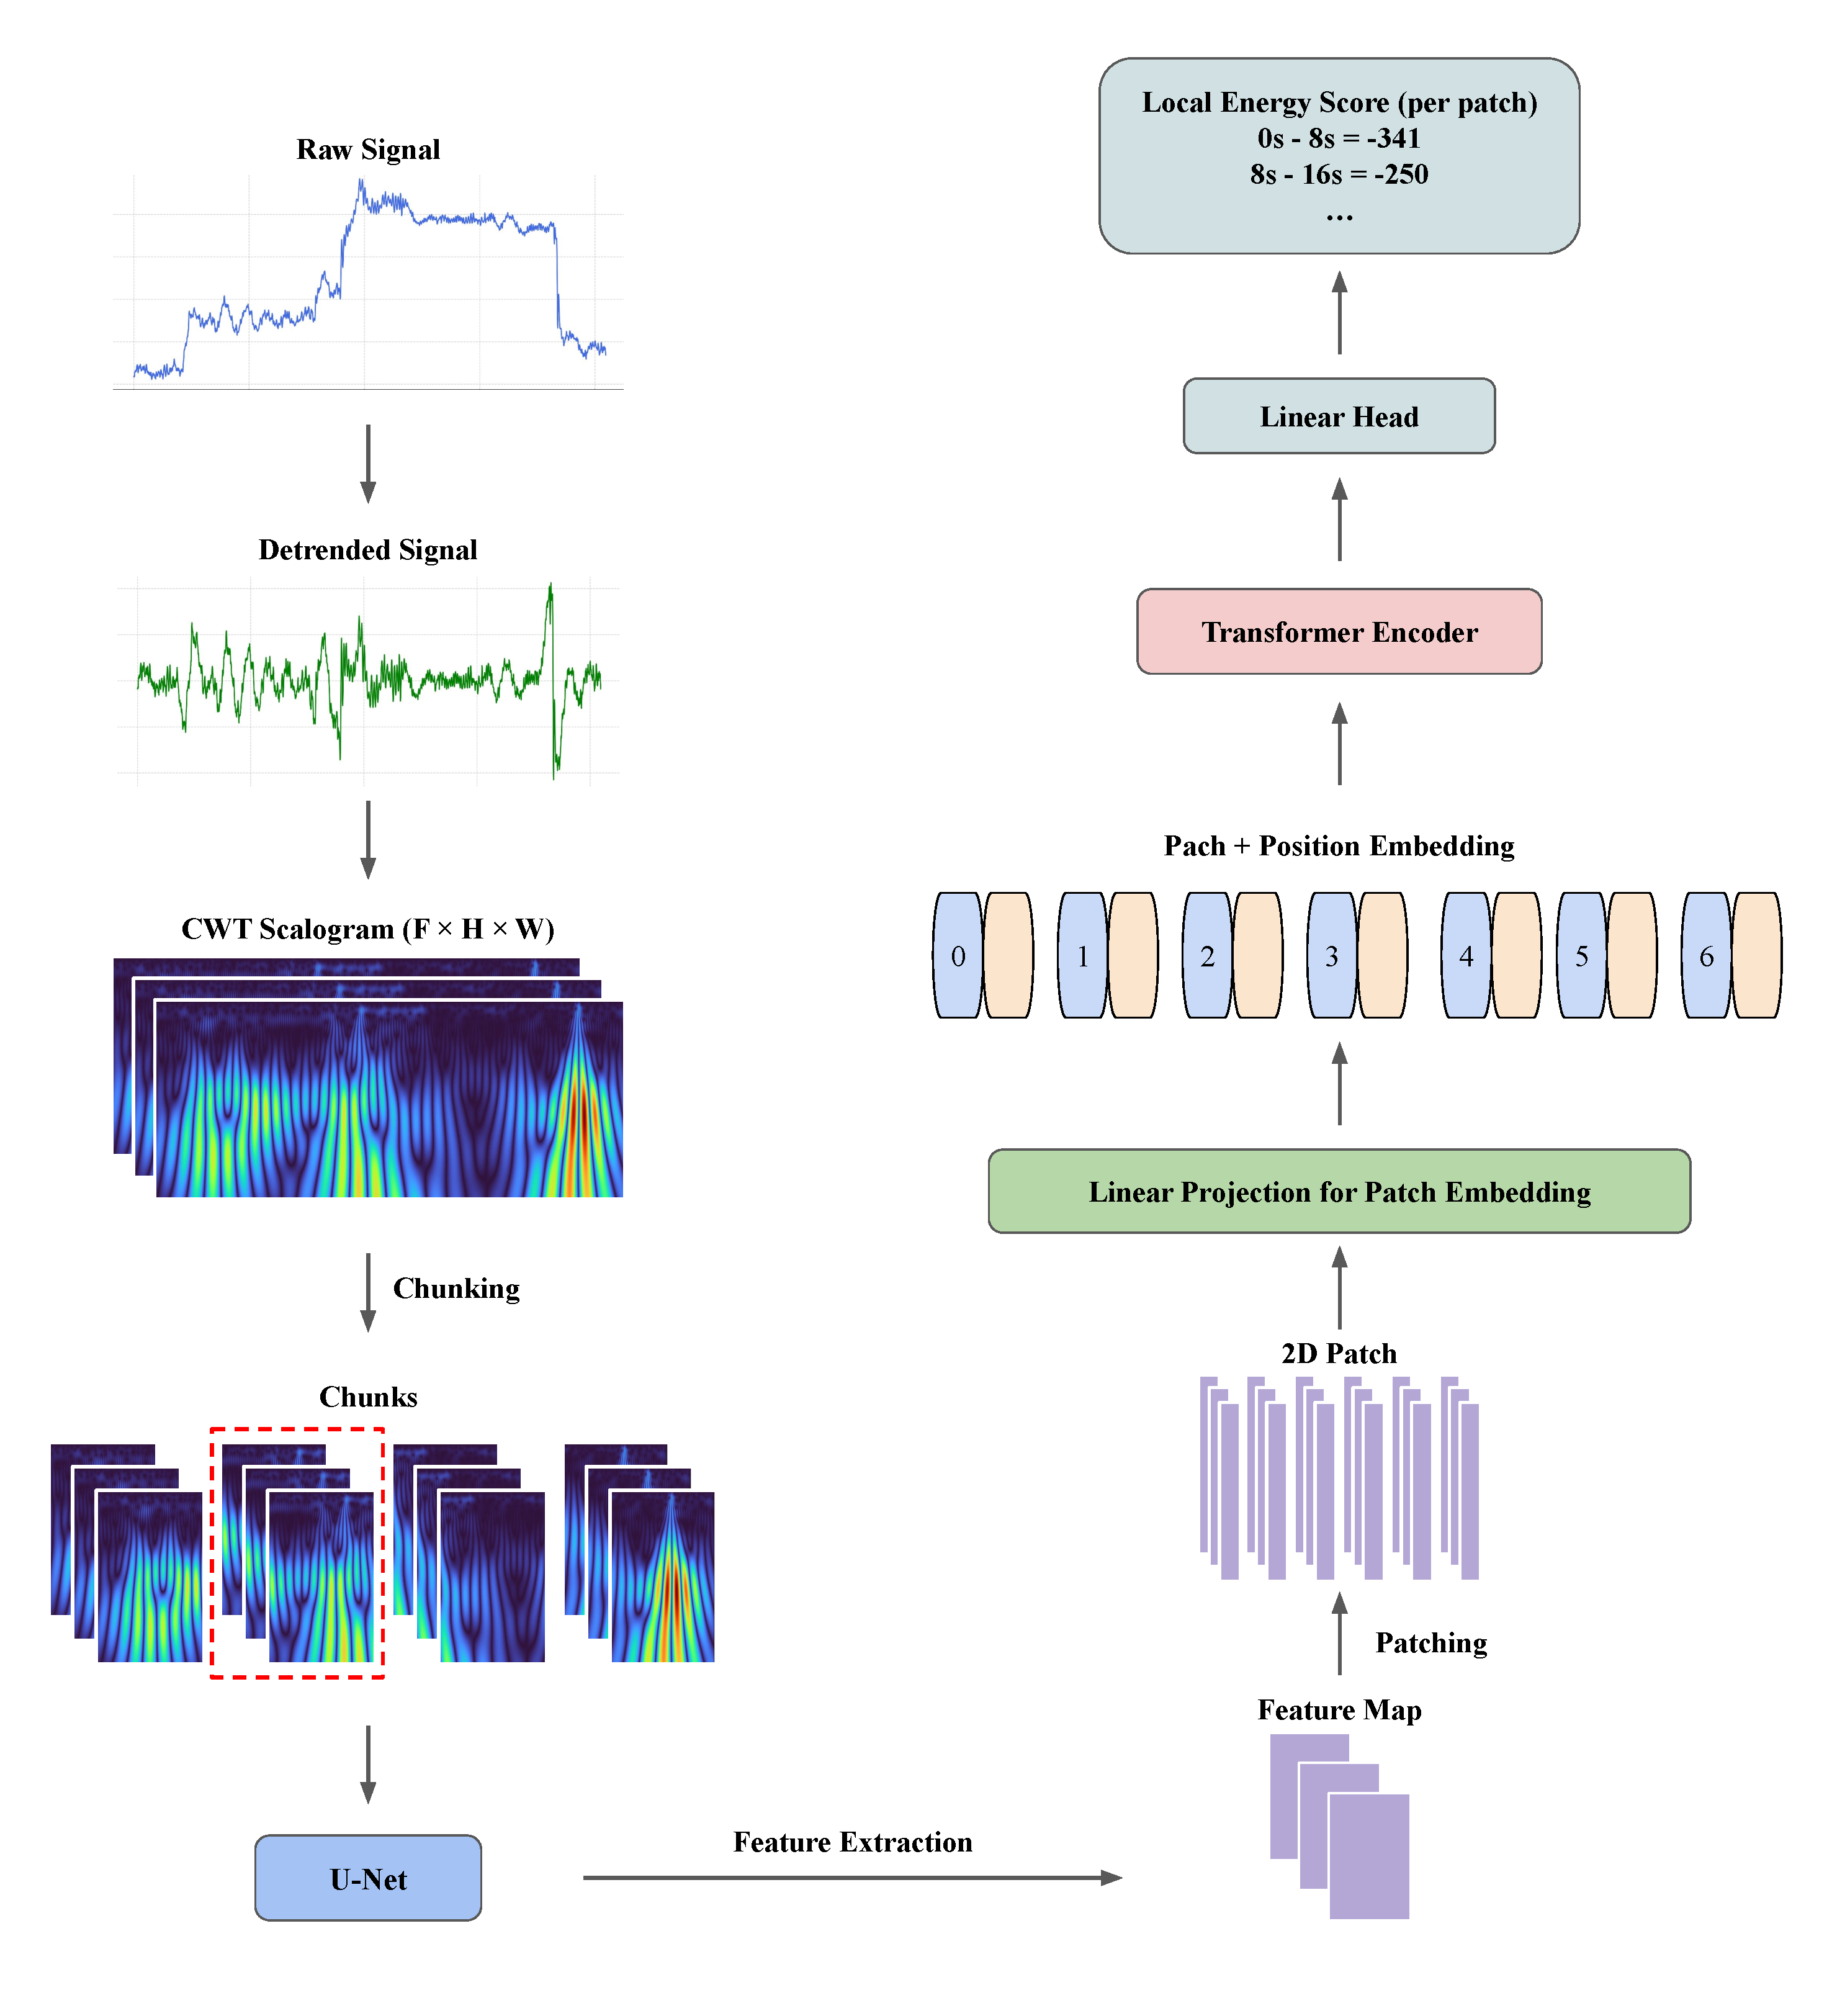
\includegraphics[width=0.8\linewidth]{figures/model_architecture.pdf}
    \caption{
    Overview of the proposed model architecture. 
    The workflow begins with raw multivariate sensor data, followed by detrending and CWT-based time–frequency transformation.
    Each chunk of the resulting multichannel scalogram is processed through a U-Net feature extractor, patch division, and a Transformer encoder.
    The model outputs localized energy scores per patch, forming interpretable energy maps that enable precise anomaly localization.}\label{fig:model_architecture}
\end{figure}

\subsection{Localized Energy-Based Model}

The core of the method is an Energy-Based Model (EBM) that learns the joint distribution of normal, multivariate sensor behavior.
An EBM defines a probability distribution via an energy function $E_\theta(x)$, parameterized by $\theta$:
\[
 p_\theta(x) = \frac{e^{-E_\theta(x)}}{Z_\theta}, \quad Z_\theta = \int e^{-E_\theta(x)} dx \]
Normal samples correspond to low-energy regions of the learned distribution, while anomalous patterns yield high energy values.

The model architecture is adapted from the Energy Matching framework proposed by \citet{balcerak2025energymatchingunifyingflow} and modified for localized anomaly detection in multichannel time–frequency representations. 
Specifically, we preserve the original energy formulation and training objective, while adjusting the encoder to process multi-feature CWT patches and to capture localized dependencies across both time and sensor dimensions.

\paragraph{Image Patching.}

The multichannel scalogram $M \in \mathbb{R}^{F \times H \times W}$ is divided into a grid of $N$ non-overlapping patches \citep{dosovitskiy_beyer_kolesnikov_weissenborn_zhai_unterthiner_dehghani_minderer_heigold_gelly_2021}:
\[
 \{p_1, p_2, \dots, p_N\}, \quad p_i \in \mathbb{R}^{F \times P_H \times P_W}, \quad N = (H / P_H) \times (W / P_W) \]
This patch-based design captures localized inter-feature and temporal–spectral dependencies, enabling the model to detect subtle, spatially confined anomalies that may not affect the entire feature set simultaneously.

\paragraph{Architecture and Local Energy Computation.}

The input multichannel scalogram is first processed by a U-Net backbone to extract hierarchical feature representations that capture spatial–temporal context across sensor channels. 
The resulting feature map is then divided into non-overlapping patches, each of which is linearly embedded and augmented with a positional encoding before being passed through a Transformer encoder $T_\theta$.

In the original Energy Matching \citep{balcerak2025energymatchingunifyingflow}, the output tokens are mean-pooled to produce a single global energy:
\[
\mathbf{z}_{\text{avg}} = \frac{1}{N} \sum_{i=1}^{N} T_\theta(p_i), \quad
E_{\text{global}} = \text{Linear}(\mathbf{z}_{\text{avg}})
\]
However, global pooling suppresses local variations critical for anomaly localization.
To retain spatial–temporal information, we remove mean-pooling and compute a local energy score per patch:\label{sec:local_energy}
\[
E_{\text{local}}(p_i) = \text{Linear}(T_\theta(p_i))
\]
This yields a set of patch-level energy values 
$\{E_{\text{local}}(p_1), \dots, E_{\text{local}}(p_N)\}$, 
providing interpretable energy maps that highlight localized deviations across both feature and time–frequency dimensions.

\subsection{Model Training via Energy Matching}

We train the EBM on normal-only data using Conditional Flow Matching (CFM). To assess the impact of additional negative-sample pressure, we also evaluate a variant that augments the objective with Contrastive Divergence (CD). The main model reported in our experiments uses CFM only; the \texttt{w/ CD Loss} variant adds CD for an ablation comparison.

\paragraph{Flow Matching Loss.}

CFM aligns the model’s velocity field $v_\theta(x, t) = -\nabla_x E_\theta(x, t)$
with a target velocity $u_t$ derived from an optimal transport path between noise and data distributions \citep{lipman_2023}:
\[ \mathcal{L}_{\text{flow}} =
\mathbb{E}_{t, p(x_t|x_1)} \left[
\| v_\theta(x_t, t) - u_t(x_t|x_1) \|^2
\right] 
\]
This regularizes the model to form a smooth energy landscape around normal samples, improving convergence stability.

\paragraph{Contrastive Divergence Loss.}\label{sec:cd_loss}

The CD loss pushes the model to assign low energy to real (normal) data and high energy to negative samples generated via Gibbs sampling:
\[ \mathcal{L}_{\text{CD}} =
\mathbb{E}_{p_{\text{data}}(x_{\text{pos}})} [E_\theta(x_{\text{pos}})] -
\mathbb{E}_{p\theta(x_{\text{neg}})} [E_\theta(x_{\text{neg}})] \]
In our main model we set $\lambda_{\text{CD}} = 0$ (FM-only); the ablation variant \texttt{w/ CD Loss} uses $\lambda_{\text{CD}} > 0$ while keeping all other settings identical.

The total objective integrates both terms with gradient regularization:
\[ \mathcal{L}_{\text{total}} =
\lambda_{\text{flow}} \mathcal{L}_{\text{flow}} +
\lambda_{\text{CD}} \mathcal{L}_{\text{CD}} +
\lambda_{\text{reg}} \| \nabla_x E_\theta(x) \|^2 \]
Unless otherwise stated, we use FM-only in all main experiments (i.e., $\lambda_{\text{CD}} = 0$); the \texttt{w/ CD Loss} ablation uses $\lambda_{\text{CD}} > 0$.
This training objective encourages the model to learn a robust energy manifold that tightly envelops the distribution of normal multivariate sensor behavior, ensuring that any deviation from this manifold results in a high energy score, indicative of an anomaly.

\subsection{Anomaly Detection and Localization}

During inference, a long multivariate signal is processed using a sliding-window strategy.

\paragraph{Chunking and Scoring.}

The full multichannel scalogram is divided into overlapping chunks of width $W_{\text{chunk}}$ and stride $S_{\text{chunk}}$.
Each chunk is passed through the trained EBM to compute patch-level energy scores.
Overlapping windows ensure that anomalies near chunk boundaries are not missed and that energy continuity is preserved across time.

\paragraph{Score Aggregation.}\label{sec:score_aggregation}

Patch-level energies from overlapping chunks are reassembled into a continuous energy tensor aligned with the time–frequency coordinates:
\[ E_{\text{timeline}}(t) = \max_{\text{chunks containing } t} E_{\text{local}}(t) \]
The max aggregation emphasizes the strongest anomaly evidence across overlapping regions, enabling high sensitivity to localized disturbances.

\paragraph{Thresholding.}

An anomaly threshold $\tau$ is determined from a validation set containing only normal data (e.g., the 99.5th percentile of energy values).
A time step $t$ is classified as anomalous if its aggregated energy exceeds the threshold:
\[
\text{Anomaly}(t) =
\begin{cases}
1, & E_{\text{timeline}}(t) > \tau \\
0, & \text{otherwise}
\end{cases}
\]
This approach provides a comprehensive anomaly timeline, enabling fine-grained localization of anomalous events across both time and feature dimensions in the original multivariate signal.


\section{Experiments and Results}

\subsection{Dataset Description}\label{sec:dataset}

This study utilizes the \textit{Three-Phase Flow Facility} dataset from Cranfield University~\citep{cao_mba_lao_samuel_2015}, which records the dynamics of a controlled two-phase (air–water) flow system. The dataset was collected from a pressurized experimental rig equipped with pipelines of varying diameters, separators, and tanks, all managed by a Delta~V SCADA system. Measurements were recorded at a sampling frequency of 1\,Hz.

A total of 24 process variables are provided, including flow rates, pressures, densities, and liquid levels. In this study, 23 soft-sensor variables were used, excluding PT417 (pressure in the 2'' line) since it is only relevant to Fault~6. The resulting multivariate time-series data are well suited for evaluating data-driven fault detection algorithms.

\paragraph{Training Data (Normal Operation).}
The training set consists of three normal-condition acquisitions (T1–T3), each representing the system under varying air and water flow conditions. These datasets were collected across 20 combinations of air and water setpoints, capturing large and small transients in both increasing and decreasing directions. This setup ensures that the training data encompass a diverse range of normal operating dynamics.

\paragraph{Testing Data (Faulty Operation).}
The testing set comprises 14 datasets corresponding to five fault types, each introduced after a period of normal operation:
\begin{enumerate}
    \item \textbf{Air line blockage} (Fault case~1.1–1.3),
    \item \textbf{Water line blockage} (Fault case~2.1–2.3),
    \item \textbf{Top separator input blockage} (Fault case~3.1–3.3),
    \item \textbf{Open direct bypass simulating a leak} (Fault case~4.1–4.3),
    \item \textbf{Slugging conditions} (Fault case~5.1–5.2).
\end{enumerate}
Each fault scenario was seeded gradually to allow observation of the fault progression over time. The sixth fault case, which involves pressurization of an isolated 2'' line, was excluded from this study because it relies on the PT417 variable, which is not included among the 23 selected sensors.

Each dataset includes clear timestamps marking fault onset and recovery, enabling quantitative evaluation of fault detection performance. In total, the dataset provides three normal-condition sequences for training and fourteen fault-condition sequences for testing.

\begin{figure}[t]
    \centering
    \begin{subfigure}[b]{0.95\linewidth}
        \centering
        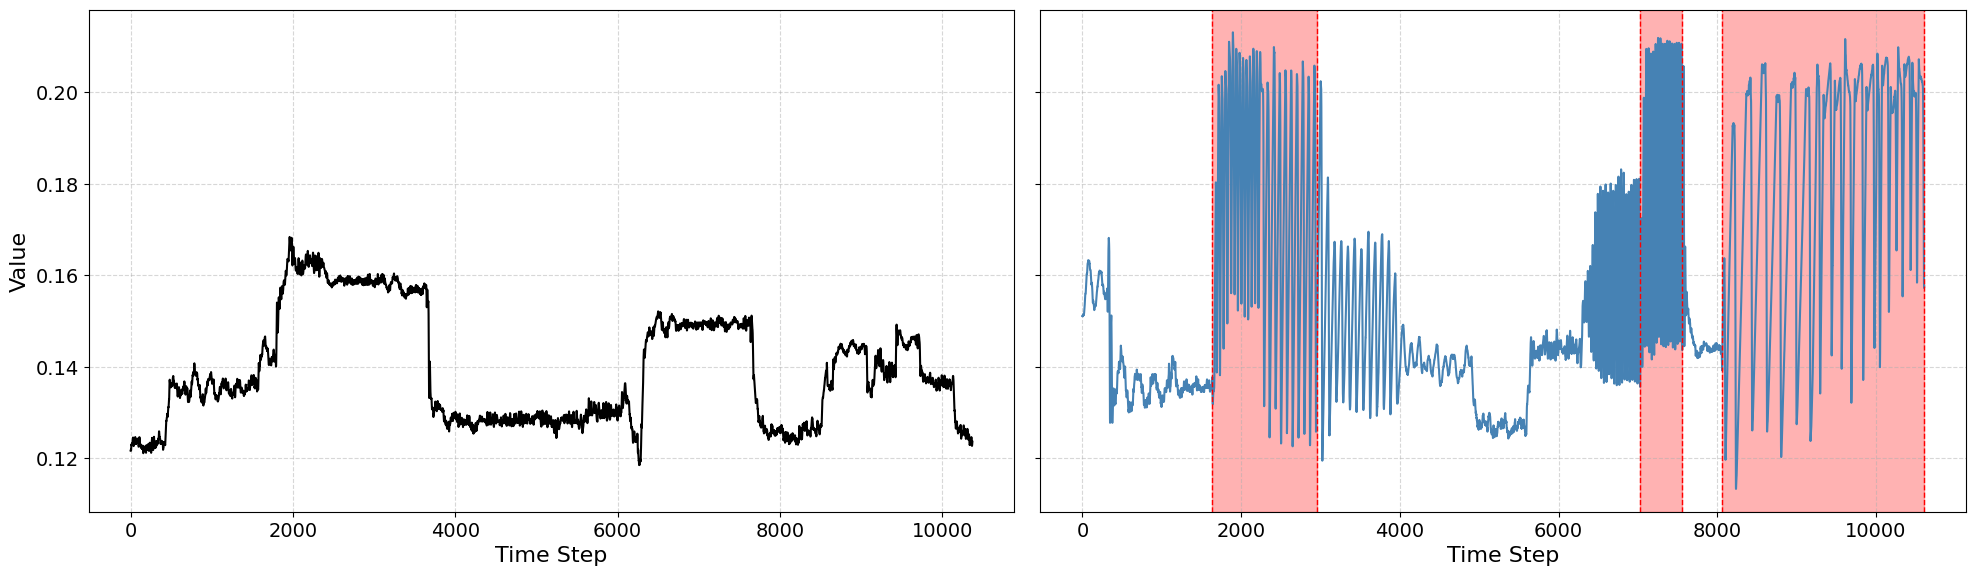
\includegraphics[width=\linewidth]{figures/comparison_F1_T1_vs_FaultyCase5_Set5_2.png}
        \subcaption{Normal (T1, Feature 1) vs. Slugging (Fault case 5.2), Feature 1}\label{fig:sub1}
    \end{subfigure}
    \vspace{1em}
    \begin{subfigure}[b]{0.95\linewidth}
        \centering
        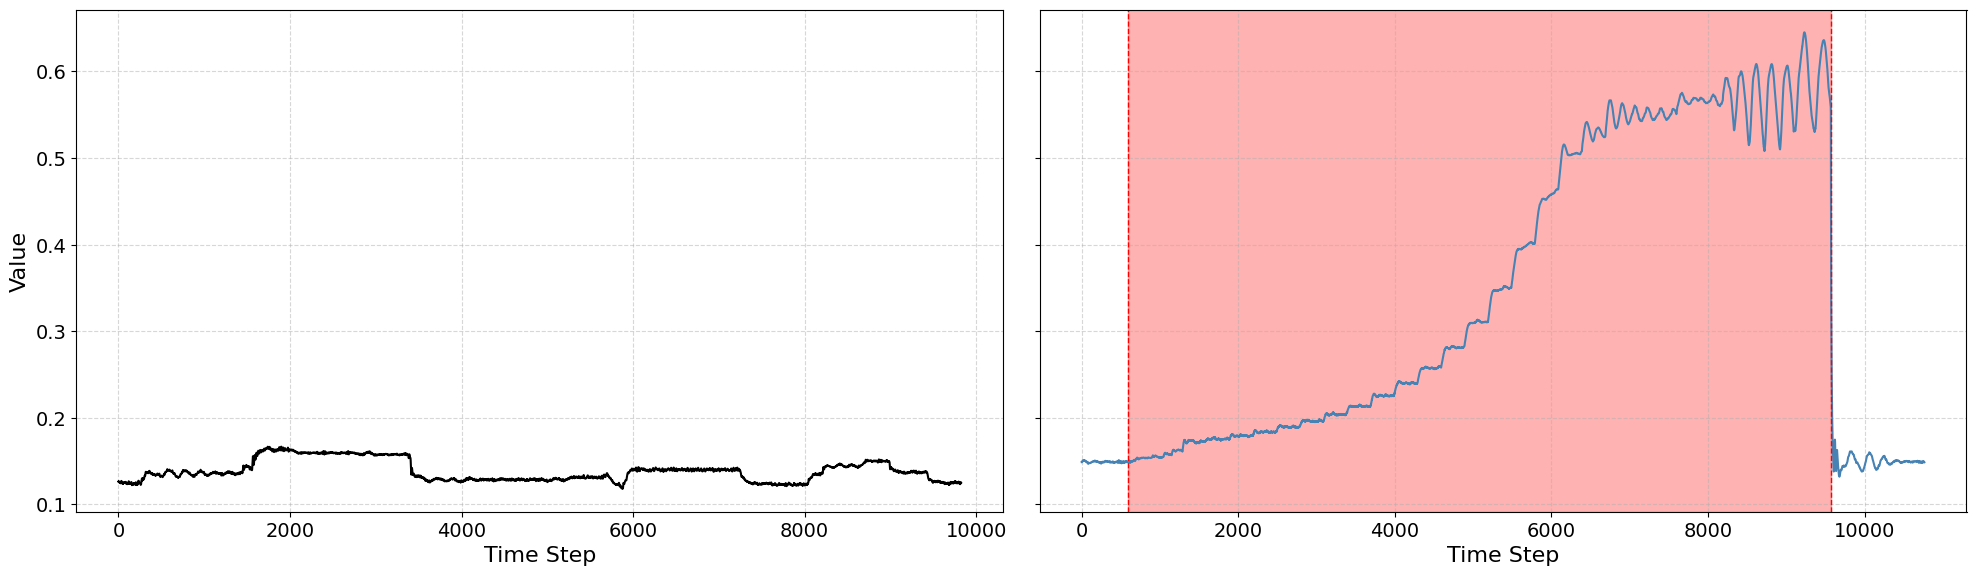
\includegraphics[width=\linewidth]{figures/comparison_F1_T2_vs_FaultyCase3_Set3_3.png}
        \subcaption{Normal (T2, Feature 1) vs. Input Blockage (Fault case 3.3), Feature 1}\label{fig:sub2}
    \end{subfigure}
    \caption{Representative examples of sensor signals for Feature 1 (pressure). Each subplot compares a normal operation signal (left) with a faulty one (right). Red-shaded regions indicate the fault intervals. (a) Compares normal operation (T1) with slugging conditions (Fault case 5.2). (b) Compares normal operation (T2) with a top separator input blockage (Fault case 3.3).}\label{fig:dataset_examples}
\end{figure}

\subsection{Quantitative Comparison with Baselines}\label{sec:model_comparison}
To rigorously assess the effectiveness of the proposed model, we compare it against two representative baselines: the LSTM-based Encoder-Decoder for Anomaly Detection (LSTM EncDec-AD) by~\citep{malhotra_ramakrishnan_anand_vig_agarwal_shroff_2016} and the Patch-based Transformer architecture (PatchTrAD) proposed by~\citep{vilhes_gasso_alaya_2025}. These models embody two complementary paradigms in unsupervised time-series anomaly detection—temporal sequence reconstruction through recurrent networks and patch-wise reconstruction-based modeling using Transformer encoders. All models are trained and evaluated on the same preprocessed Multiphase Flow Process (MFP) dataset under identical experimental settings.
Performance is assessed using two principal metrics: F1 Score and ROC-AUC. The F1 Score quantifies the balance between precision and recall under a fixed threshold, while ROC-AUC provides a threshold-independent measure of discriminative capability. Together, these metrics capture complementary aspects of anomaly detection performance. Table~\ref{tab:model_comparison_f1_auc} summarizes the results across all fault cases, with bold values indicating the best-performing model for each metric and scenario.
\begin{table*}[t] 
 \centering 
 \caption{Performance comparison of baseline and proposed models across all fault cases in the MFP dataset, focusing on F1 Score and ROC-AUC. Bold values indicate the best performance for each metric.}\label{tab:model_comparison_f1_auc}
 \resizebox{0.9\textwidth}{!}{
 \begin{tabular}{lrr|rr|rr}
 \toprule
 \multirow{2}{*}{\textbf{Fault Case}} & \multicolumn{2}{c|}{\textbf{LSTM EncDec-AD \citep{malhotra_ramakrishnan_anand_vig_agarwal_shroff_2016}}} & \multicolumn{2}{c|}{\textbf{PatchTrAD \citep{vilhes_gasso_alaya_2025}}} & \multicolumn{2}{c}{\textbf{Proposed (Ours)}} \\
 \cmidrule(lr){2-3} \cmidrule(lr){4-5} \cmidrule(lr){6-7}
 & F1 & ROC-AUC & F1 & ROC-AUC & F1 & ROC-AUC \\
 \midrule
FaultyCase1\_Set1\_1 & 0.64 & 0.61 & 0.49 & 0.68 & \textbf{0.78} & \textbf{0.74} \\
FaultyCase1\_Set1\_2 & 0.56 & 0.61 & 0.50 & 0.54 & \textbf{0.86} & \textbf{0.65} \\
FaultyCase1\_Set1\_3 & 0.55 & 0.42 & 0.37 & 0.56 & \textbf{0.84} & \textbf{0.65} \\
FaultyCase2\_Set2\_1 & 0.33 & 0.48 & 0.00 & \textbf{0.52} & \textbf{0.45} & 0.37 \\
FaultyCase2\_Set2\_2 & \textbf{0.26} & 0.18 & 0.00 & 0.36 & 0.03 & \textbf{0.49} \\
FaultyCase2\_Set2\_3 & 0.24 & 0.17 & 0.01 & 0.36 & \textbf{0.66} & \textbf{0.40} \\
FaultyCase3\_Set3\_1 & \textbf{0.98} & \textbf{0.99} & \textbf{0.98} & 0.94 & 0.89 & 0.81 \\
FaultyCase3\_Set3\_2 & \textbf{0.95} & \textbf{0.74} & 0.69 & 0.54 & 0.74 & 0.45 \\
FaultyCase3\_Set3\_3 & 0.96 & \textbf{0.99} & \textbf{0.98} & 0.92 & 0.91 & 0.37 \\
FaultyCase4\_Set4\_1 & \textbf{0.89} & \textbf{0.80} & 0.59 & 0.77 & 0.85 & 0.71 \\
FaultyCase4\_Set4\_2 & 0.47 & \textbf{0.61} & 0.26 & 0.36 & \textbf{0.81} & \textbf{0.61} \\
FaultyCase4\_Set4\_3 & 0.70 & 0.41 & 0.36 & 0.39 & \textbf{0.90} & \textbf{0.67} \\
FaultyCase5\_Set5\_1 & \textbf{0.69} & 0.59 & 0.59 & 0.66 & 0.57 & \textbf{0.94} \\
FaultyCase5\_Set5\_2 & 0.84 & \textbf{0.97} & \textbf{0.87} & 0.96 & 0.59 & 0.96 \\
 \midrule 
 \textbf{Overall Average} & \textbf{0.77} & \textbf{0.77} & 0.67 & 0.73 & 0.76 & 0.60 \\
 \bottomrule 
 \end{tabular}}
 \end{table*}

Overall, the comparison reveals that no single model consistently dominates across all scenarios. The LSTM EncDec-AD performs particularly well in FaultyCase3 and FaultyCase4, achieving near-perfect F1 and ROC-AUC scores in some subsets, reflecting its strength in capturing longer-term temporal dependencies in quasi-periodic faults. In contrast, its performance notably declines in FaultyCase2, suggesting difficulty handling less predictable or irregular signals.
The PatchTrAD model exhibits more stable results across fault conditions, often achieving moderate to high ROC-AUC values, particularly in FaultyCase3 and FaultyCase5, where localized representations help discriminate subtle variations in temporal patterns. However, it occasionally underperforms in F1 Score when threshold calibration becomes challenging due to overlapping normal–fault distributions.
The proposed model achieves competitive or leading F1 and ROC-AUC values in several fault cases (e.g., FaultyCase1 and FaultyCase4), indicating its effectiveness in detecting deviations from the learned distribution of normal behavior. Nevertheless, its performance fluctuates in certain subsets such as FaultyCase3, suggesting that while the patch-level representations effectively capture local anomalies, they may be less robust in globally periodic patterns compared to recurrent baselines.

\begin{figure}[t]
    \centering
    \begin{subfigure}[b]{0.32\textwidth}
        \centering
        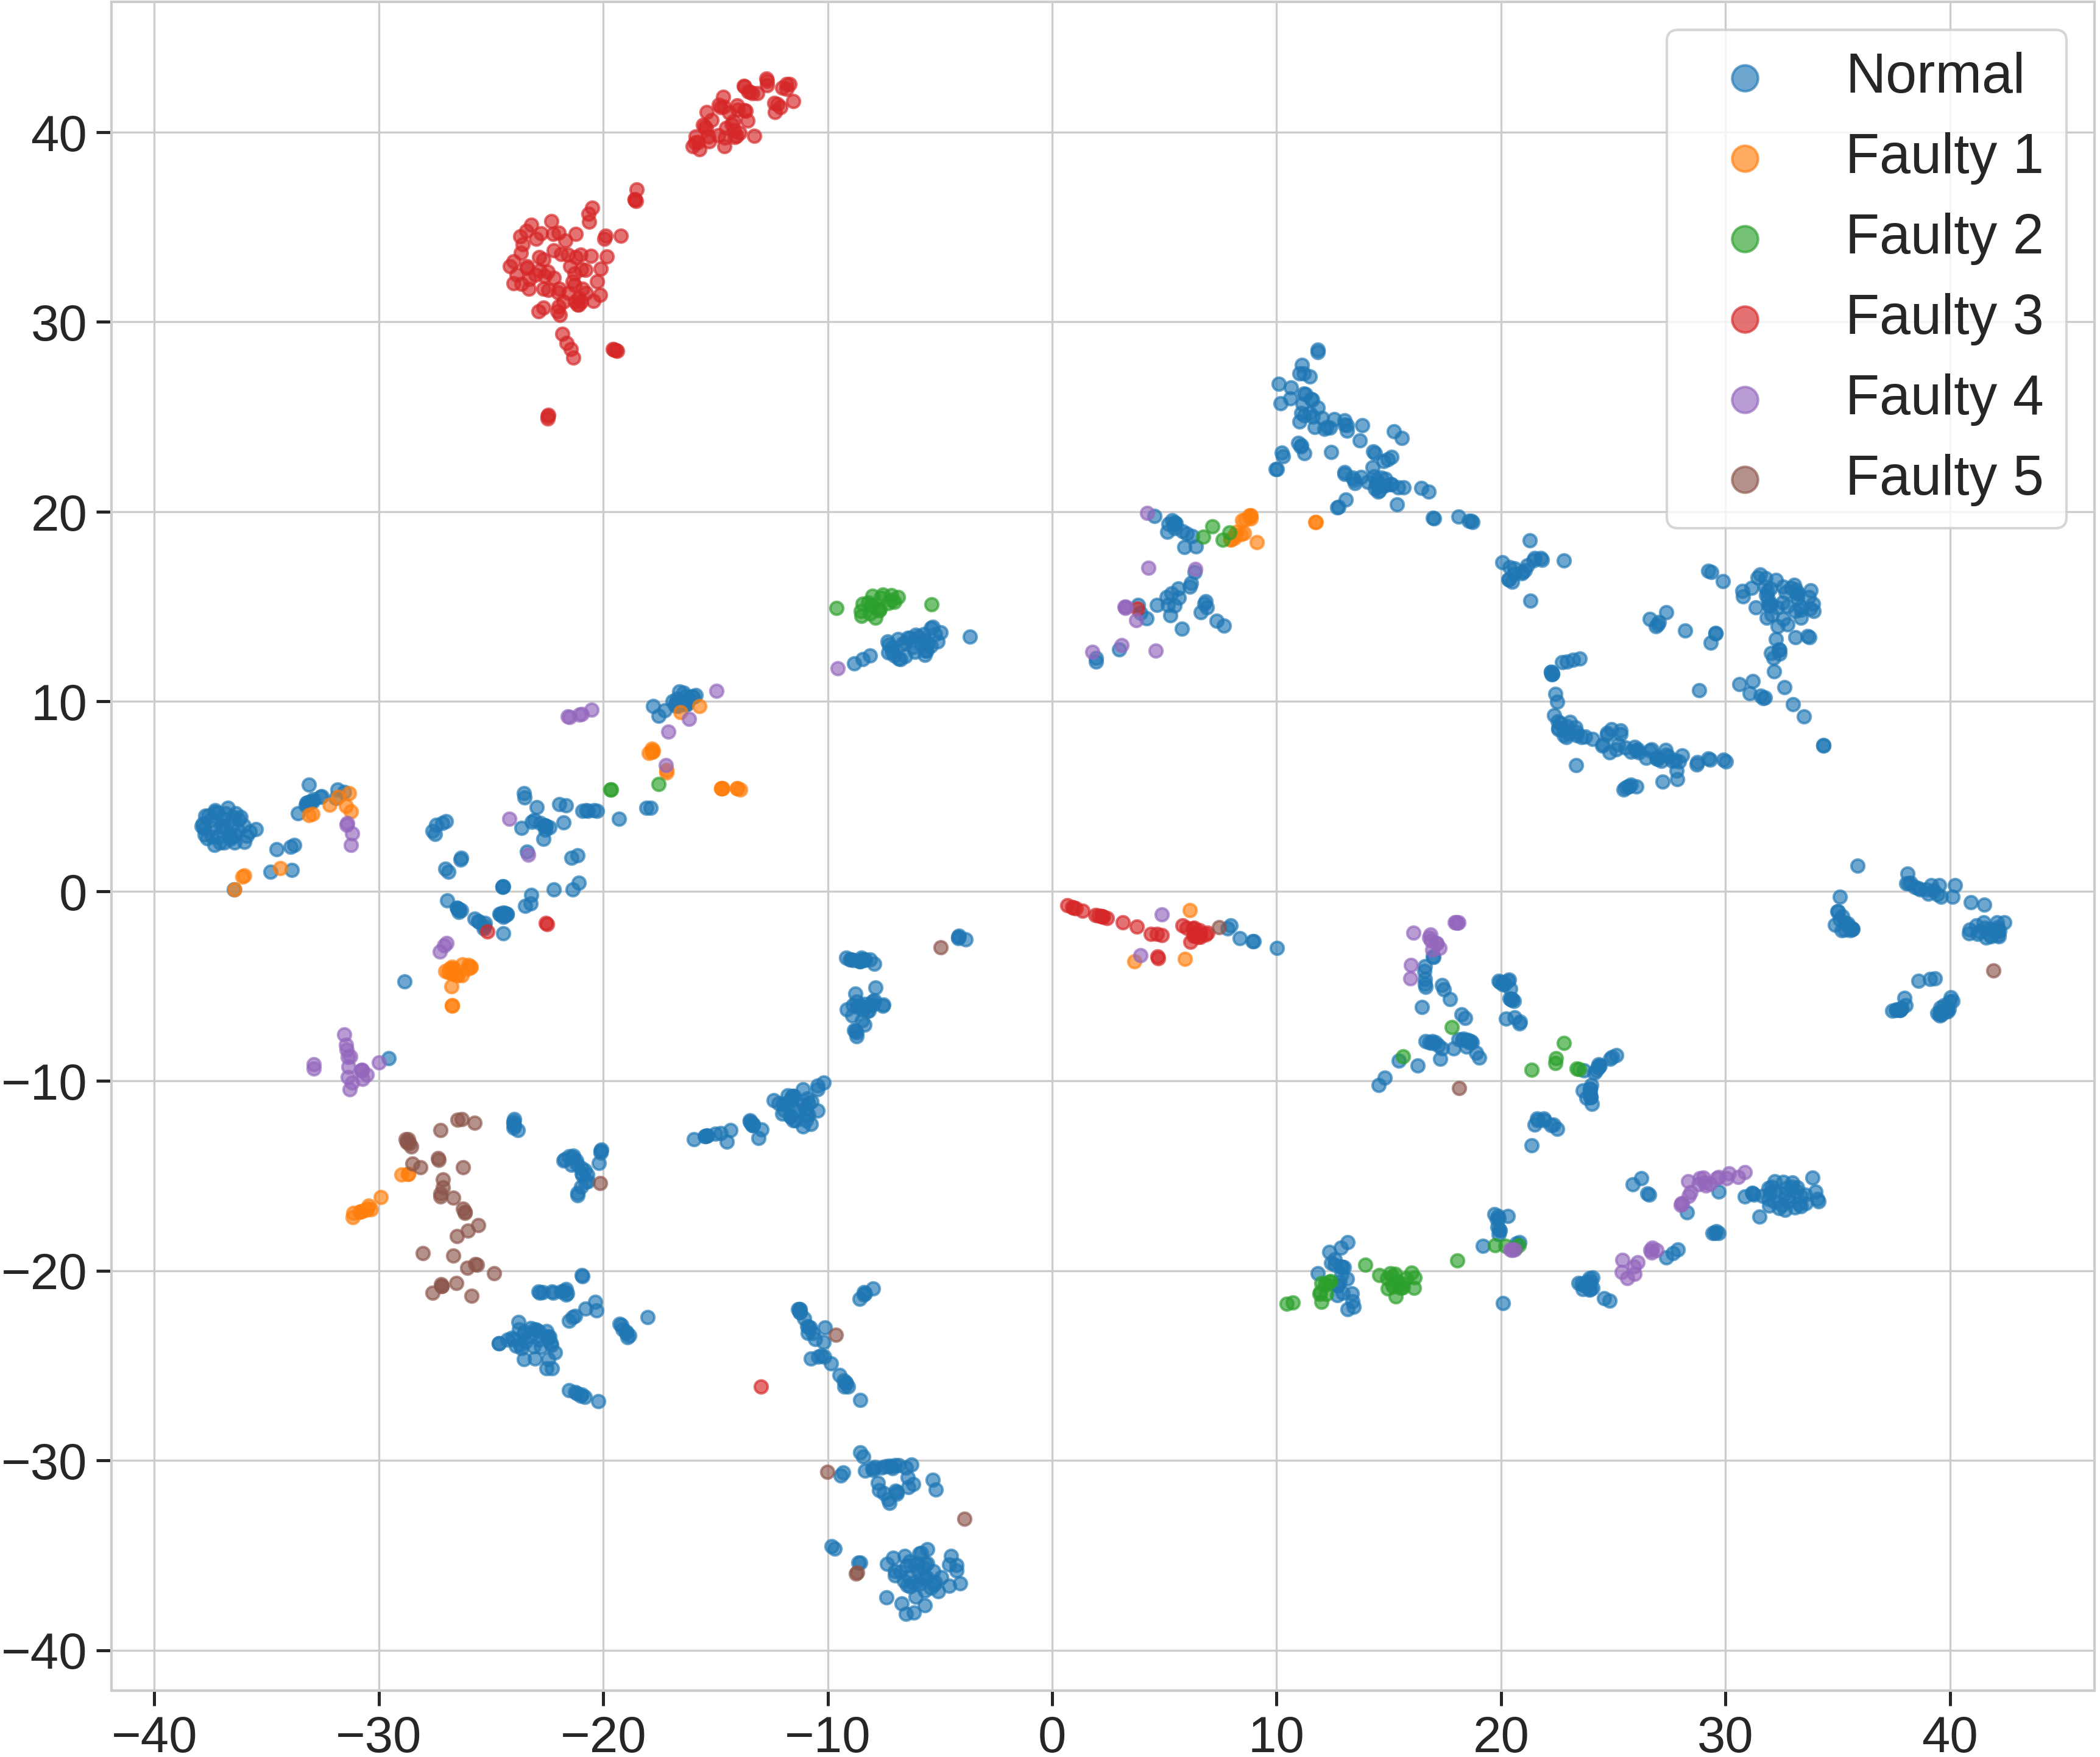
\includegraphics[width=\textwidth]{figures/tsne_lstm_autoencoder.png}
        \caption{LSTM EncDec-AD}\label{fig:tsne_lstm}
    \end{subfigure}
    \hfill
    \begin{subfigure}[b]{0.32\textwidth}
        \centering
        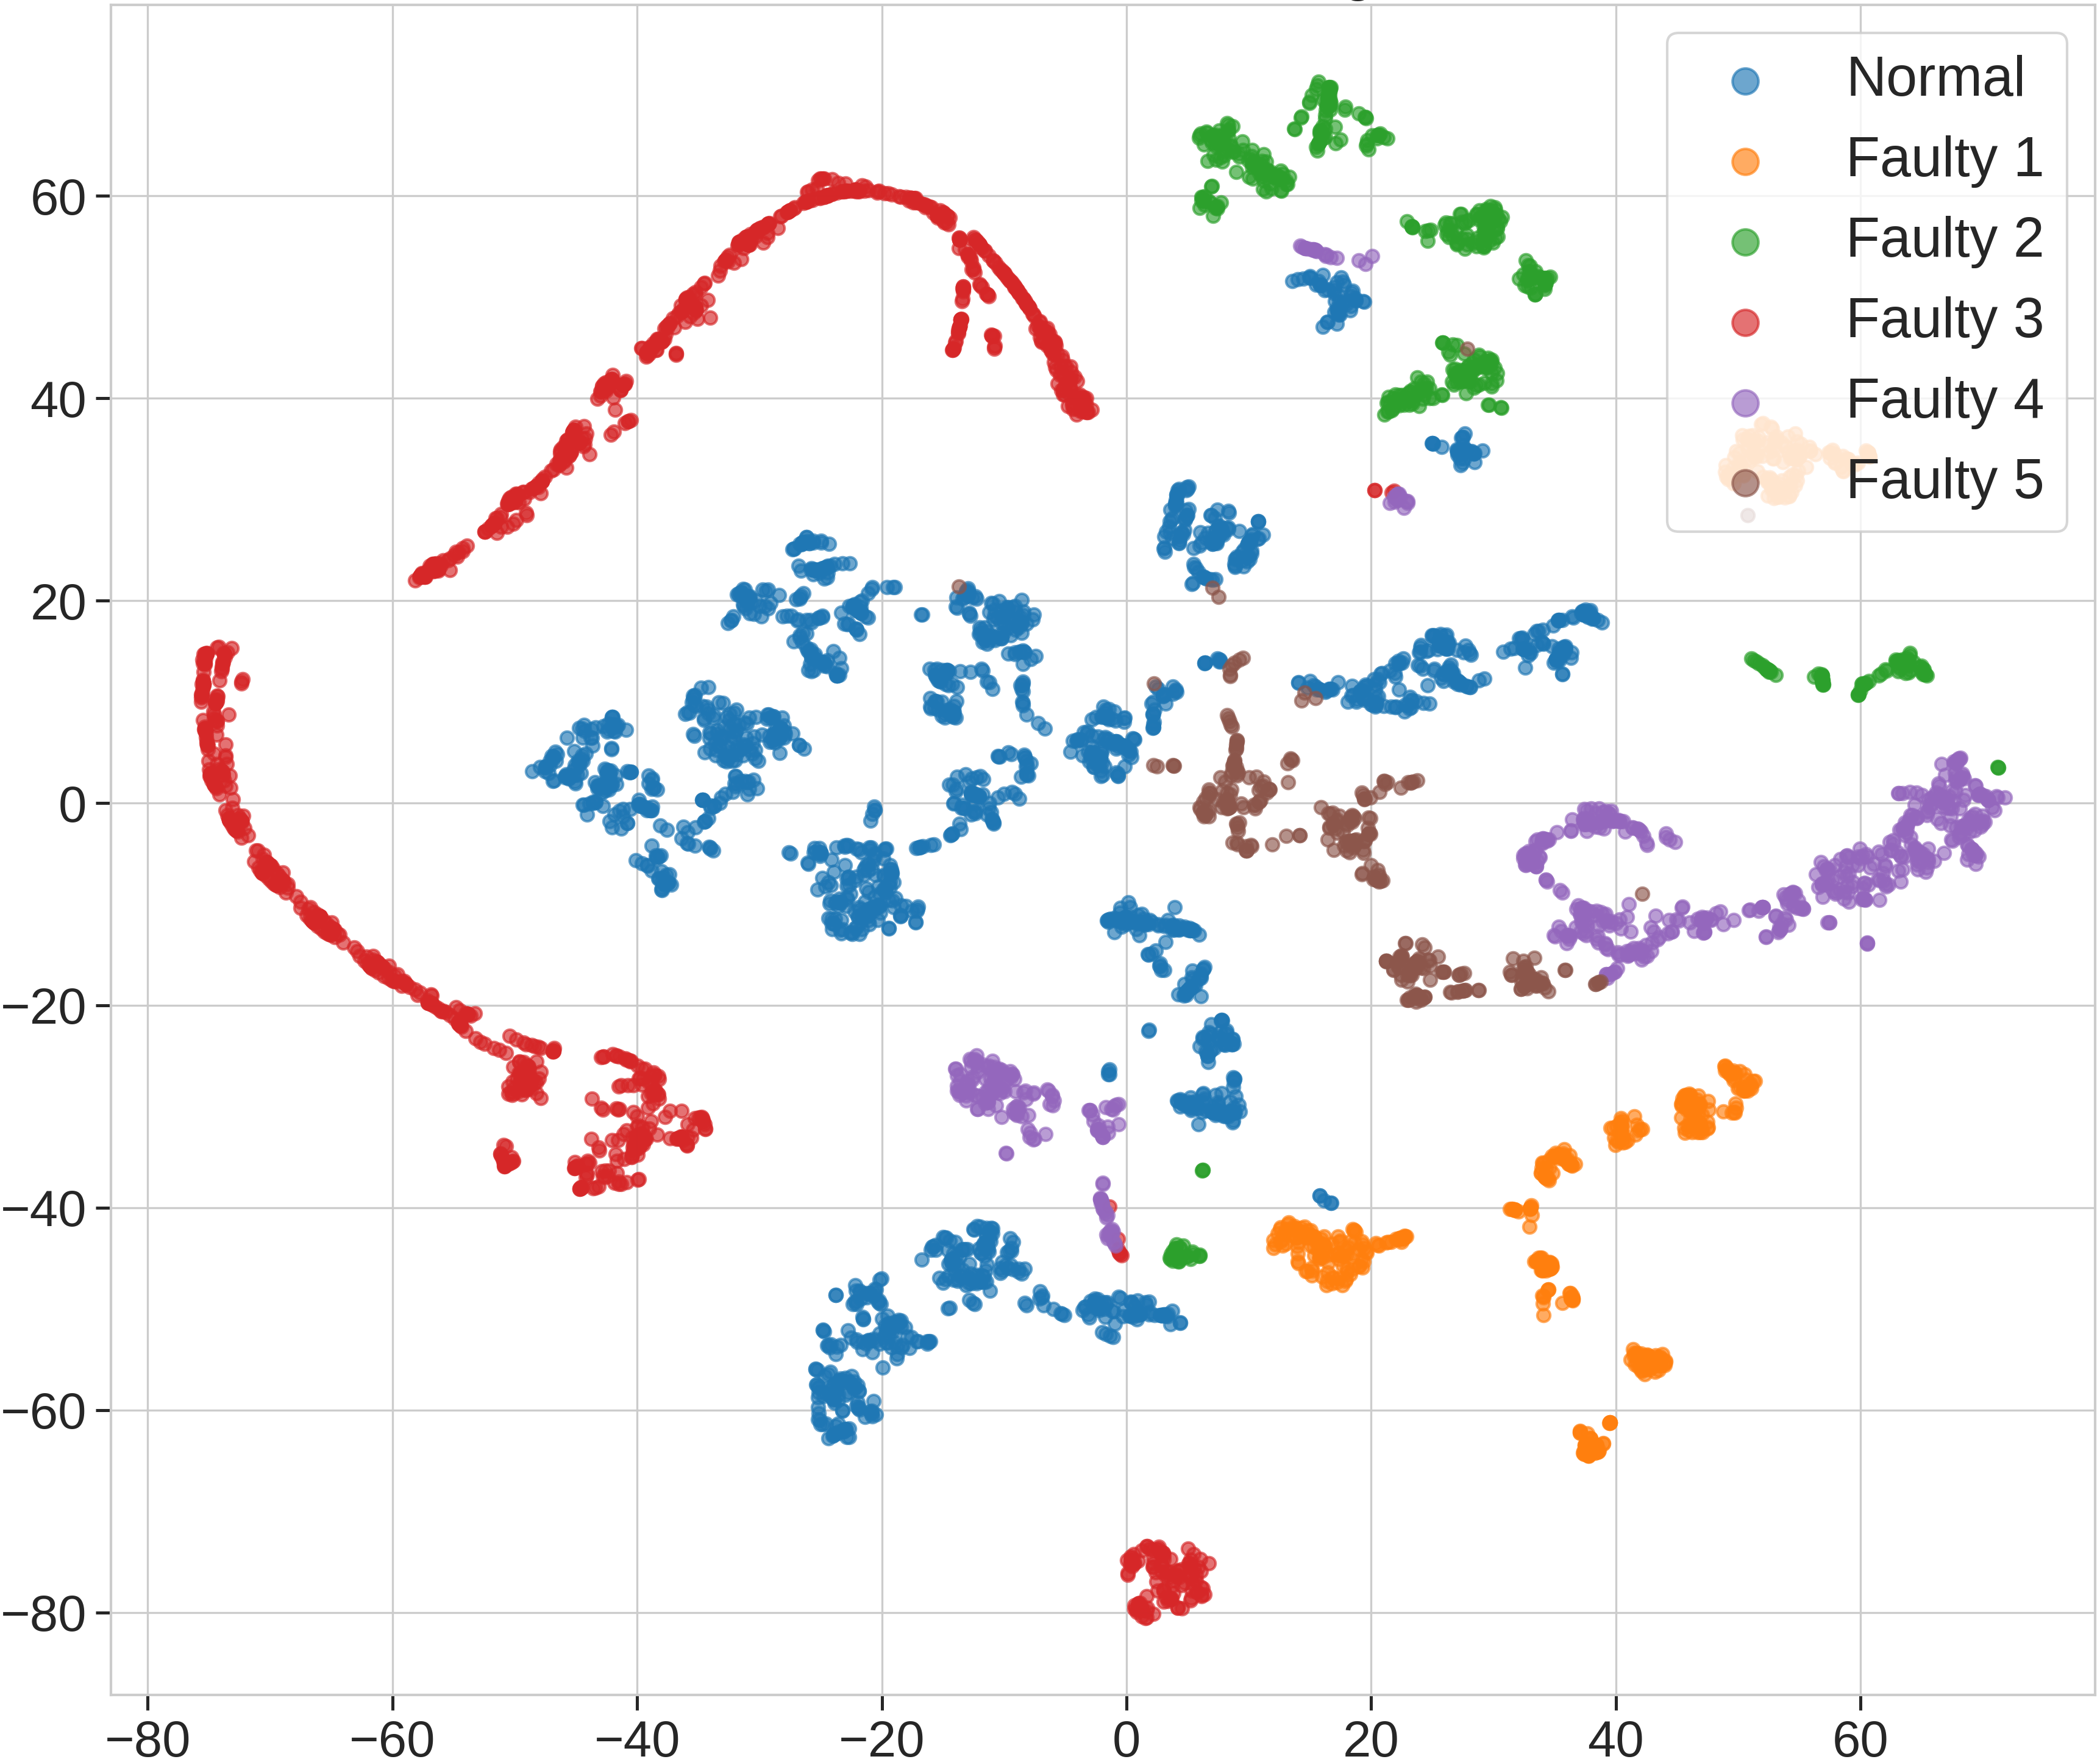
\includegraphics[width=\textwidth]{figures/tsne_patchtrad.png}
        \caption{PatchTrAD}\label{fig:tsne_patchtrad}
    \end{subfigure}
    \hfill
    \begin{subfigure}[b]{0.32\textwidth}
        \centering
        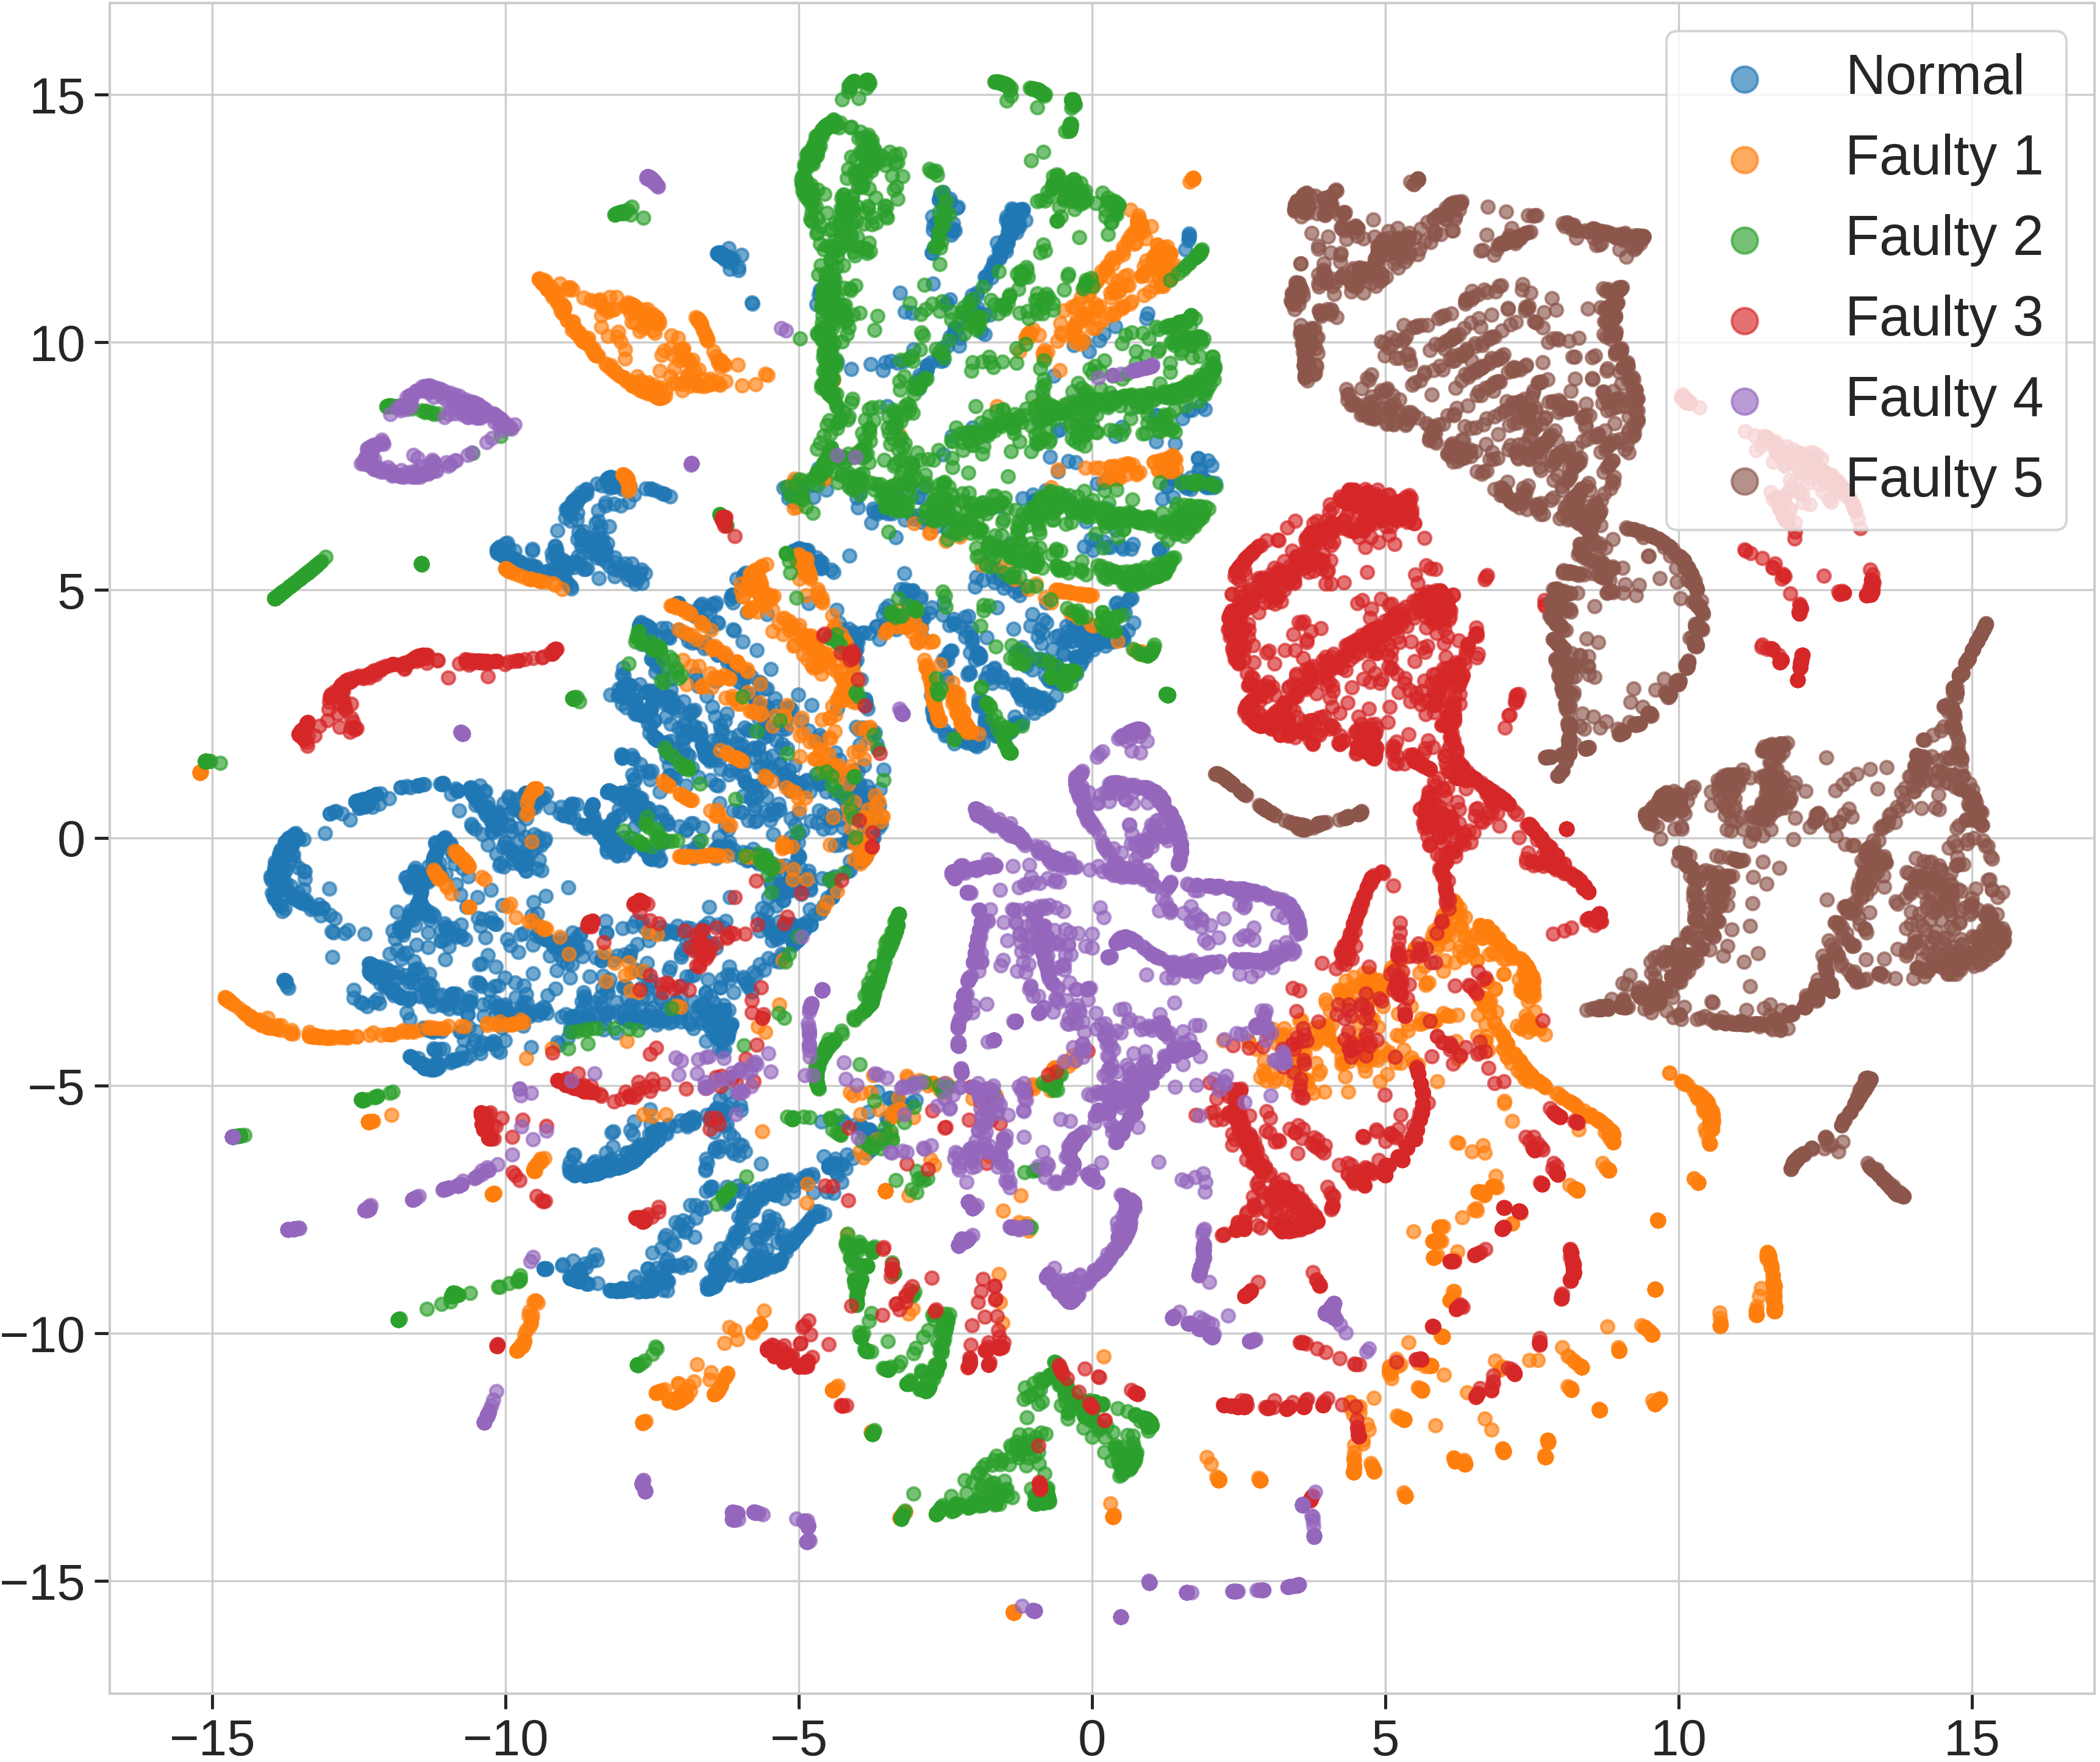
\includegraphics[width=\textwidth]{figures/tsne_patch_visualization.png}
        \caption{Proposed Model}\label{fig:tsne_proposed}
    \end{subfigure}
    \caption{Comparative t-SNE visualization of latent feature spaces from (a) the LSTM EncDec-AD, (b) PatchTrAD, and (c) the proposed model. Each point is a time-series segment colored by its true label (Normal or Fault types 1-5). The visualization highlights the complementary strengths of the models: while the baseline LSTM EncDec-AD (a) effectively isolates FaultyCase 3, the proposed model (c) uniquely excels at separating the complex patterns of FaultyCase 5 from normal behavior, even though some overlap persists in other classes. This demonstrates our model's capability to learn discriminative features for specific, challenging anomaly signatures.}\label{fig:tsne_comparison}
\end{figure}

To further interpret these quantitative findings, we visualize the latent feature distributions using t-distributed Stochastic Neighbor Embedding (t-SNE) in Fig.\ref{fig:tsne_comparison}. Each point represents a segment of the time series, color-coded by its true label (Normal or Faulty 1–5).
The LSTM EncDec-AD (Fig.\ref{fig:tsne_lstm}) exhibits considerable overlap between normal and faulty representations, except for FaultyCase 3, which forms a distinct cluster—consistent with its strong numerical performance in Table~\ref{tab:model_comparison_f1_auc}.
The PatchTrAD model (Fig.\ref{fig:tsne_patchtrad}) demonstrates improved separation between normal and fault samples, particularly for FaultyCase 3, though partial overlap remains for FaultyCase 4 and FaultyCase 5.
In contrast, the proposed model (Fig.\ref{fig:tsne_proposed}) clearly distinguishes FaultyCase 5 from normal samples, aligning with its outstanding ROC-AUC score in that scenario. However, partial intermixing persists among FaultyCase 1–4 and normal representations, indicating potential room for refinement in feature disentanglement for overlapping fault types.

Collectively, these results reveal a clear architectural trade-off: the recurrent LSTM is superior for globally periodic faults, while the patch-based PatchTrAD is effective for localized events. Our proposed energy-based model demonstrates a powerful synthesis, achieving a balanced performance across diverse faults while uniquely excelling at complex, high-frequency anomalies like FaultyCase 5.

\subsection{Ablation Study}\label{sec:ablation_study}
To validate our core design choices, we conducted an extensive ablation study evaluating the impact of architectural and methodological variations on overall performance. We compare our full proposed model, \textbf{ScaloVit-EBM}, against four ablated variants:
\begin{itemize}
    \item \textbf{w/o Detrending}: Removes the moving-average detrending step (Section~\ref{sec:detrending}) from the preprocessing pipeline.
    \item \textbf{Global-ViT (Image-Based Scoring)}: Replaces the per-patch scoring mechanism (Section~\ref{sec:local_energy}) with a global score, testing the value of localized energy computation.
    \item \textbf{w/ CD Loss}: Trained with the Contrastive Divergence (CD) loss component (Section~\ref{sec:cd_loss}) to evaluate its contribution.
    \item \textbf{Mean Aggregation}: Replaces the \texttt{max} aggregation strategy (Section~\ref{sec:score_aggregation}) with \texttt{mean} averaging for reconstructing scores.
\end{itemize}

\begin{table*}[h!]
\centering
\caption{Detailed ablation study results across all fault cases. For each case, we report F1 Score and ROC-AUC. Bold values indicate the best-performing model variant for that metric in that row.}\label{tab:ablation_study_detailed}
\resizebox{\textwidth}{!}{
\begin{tabular}{lrr|rr|rr|rr|rr}
\toprule
\multirow{2}{*}{\textbf{Fault Case}} & \multicolumn{2}{c|}{\textbf{ScaloVit-EBM (FM-only)}} & \multicolumn{2}{c|}{\textbf{w/o Detrending}} & \multicolumn{2}{c|}{\textbf{Global-ViT}} & \multicolumn{2}{c|}{\textbf{w/ CD Loss}} & \multicolumn{2}{c}{\textbf{Mean Aggregation}} \\
\cmidrule(lr){2-3} \cmidrule(lr){4-5} \cmidrule(lr){6-7} \cmidrule(lr){8-9} \cmidrule(lr){10-11}
 & F1 & ROC-AUC & F1 & ROC-AUC & F1 & ROC-AUC & F1 & ROC-AUC & F1 & ROC-AUC \\
\midrule
FaultyCase1\_Set1\_1 & \textbf{0.78} & \textbf{0.74} & 0.75 & 0.60 & 0.77 & 0.71 & 0.77 & 0.70 & 0.63 & 0.53 \\
FaultyCase1\_Set1\_2 & \textbf{0.86} & \textbf{0.65} & 0.83 & 0.59 & \textbf{0.86} & 0.62 & \textbf{0.86} & \textbf{0.65} & 0.71 & 0.51 \\
FaultyCase1\_Set1\_3 & 0.84 & \textbf{0.65} & 0.82 & 0.59 & 0.84 & \textbf{0.65} & \textbf{0.85} & 0.64 & 0.68 & 0.54 \\
FaultyCase2\_Set2\_1 & 0.45 & 0.37 & 0.00 & 0.04 & 0.45 & \textbf{0.41} & \textbf{0.46} & 0.38 & 0.16 & 0.27 \\
FaultyCase2\_Set2\_2 & 0.03 & 0.49 & 0.57 & 0.36 & 0.61 & \textbf{0.55} & \textbf{0.78} & 0.45 & 0.01 & 0.38 \\
FaultyCase2\_Set2\_3 & 0.66 & 0.40 & \textbf{0.77} & 0.24 & 0.73 & \textbf{0.46} & 0.75 & 0.35 & 0.06 & 0.27 \\
FaultyCase3\_Set3\_1 & \textbf{0.89} & 0.81 & \textbf{0.89} & 0.64 & \textbf{0.89} & \textbf{0.85} & \textbf{0.89} & 0.67 & \textbf{0.89} & 0.46 \\
FaultyCase3\_Set3\_2 & 0.74 & \textbf{0.45} & 0.69 & 0.29 & 0.67 & 0.42 & \textbf{0.76} & 0.43 & 0.62 & 0.38 \\
FaultyCase3\_Set3\_3 & \textbf{0.91} & \textbf{0.37} & \textbf{0.91} & 0.34 & \textbf{0.91} & 0.27 & \textbf{0.91} & 0.34 & \textbf{0.91} & 0.17 \\
FaultyCase4\_Set4\_1 & \textbf{0.85} & \textbf{0.71} & \textbf{0.85} & 0.61 & \textbf{0.85} & 0.43 & \textbf{0.85} & 0.52 & 0.65 & 0.53 \\
FaultyCase4\_Set4\_2 & \textbf{0.81} & 0.61 & \textbf{0.81} & 0.54 & \textbf{0.81} & \textbf{0.70} & \textbf{0.81} & 0.62 & \textbf{0.81} & 0.16 \\
FaultyCase4\_Set4\_3 & \textbf{0.90} & \textbf{0.67} & \textbf{0.90} & 0.26 & \textbf{0.90} & \textbf{0.67} & \textbf{0.90} & 0.40 & \textbf{0.90} & 0.26 \\
FaultyCase5\_Set5\_1 & \textbf{0.57} & \textbf{0.94} & \textbf{0.57} & \textbf{0.94} & \textbf{0.57} & 0.65 & \textbf{0.57} & 0.92 & \textbf{0.57} & 0.90 \\
FaultyCase5\_Set5\_2 & 0.59 & \textbf{0.96} & 0.59 & \textbf{0.96} & 0.60 & 0.92 & 0.59 & 0.95 & \textbf{0.63} & 0.95 \\
\midrule
\textbf{Overall Average} & 0.76 & \textbf{0.60} & 0.76 & 0.57 & 0.77 & 0.59 & \textbf{0.78} & 0.59 & 0.69 & 0.55 \\
\bottomrule
\end{tabular}}
\end{table*} 

\paragraph{Analysis of Architectural Components.} The detailed results in Table~\ref{tab:ablation_study_detailed} reveal several key insights. The clearest findings relate to the preprocessing and aggregation steps. The choice of aggregation strategy proves critical, as the Mean Aggregation model yields the lowest overall ROC-AUC score of all variants (0.55). A score this close to random chance (0.5) indicates that mean averaging dilutes localized, high-energy deviations, making the normal and faulty distributions nearly indistinguishable. This strongly validates our use of max aggregation to preserve these critical signatures. Similarly, removing the preprocessing step in the w/o Detrending model causes the overall ROC-AUC to fall from 0.60 to 0.57. The performance degradation is particularly severe in certain scenarios, such as \texttt{FaultyCase2\_Set2\_1} and \texttt{FaultyCase4\_Set4\_3}, where the ROC-AUC collapses to near-random levels (0.04 and 0.26, respectively). This suggests that without removing the natural baseline variations present in the raw signals, the model struggles to learn a discriminative energy function that can reliably separate anomalous patterns from normal operational fluctuations. Together, these findings confirm that both detrending and max aggregation are essential for learning a robust and discriminative energy function.

\paragraph{Value of Localized Scoring.} The Global-ViT ablation, which replaces per-patch scoring with a single global energy score per chunk, directly tests our core architectural hypothesis. At first glance, its overall performance appears comparable to the full model, with a slightly higher F1 score (0.77) and a nearly identical ROC-AUC (0.59). However, this aggregate view masks a critical weakness. For FaultyCase5 (slugging), the performance of the Global-ViT model collapses, with its ROC-AUC score dropping from 0.94 to 0.65 in one instance. This demonstrates that while a global energy score is sufficient for many fault types, the localized, per-patch scoring mechanism is indispensable for correctly identifying spatially complex anomalies like slugging, thus validating our proposed architecture.

\paragraph{Impact of Loss Function.} The comparison between the top-performing variants reveals a crucial design trade-off. Our main proposed model, ScaloVit-EBM (FM-only), achieves the highest overall ROC-AUC (0.60), indicating the best intrinsic class separability. In an ablation study, we introduced a computationally intensive Contrastive Divergence (CD) loss (the w/ CD Loss model). Interestingly, this variant achieved the highest overall F1 score (0.78). This presents a trade-off between performance metrics and computational cost. While adding the CD loss can create a decision boundary that is highly effective for a single-threshold detector (leading to a higher aggregate F1), it does so at the cost of a slight decrease in overall class separability (lower ROC-AUC) and a significant increase in training complexity. The strong performance of our proposed model without this extra loss validates our design choice for a more efficient architecture that maintains superior class-separation capabilities.

\paragraph{Impact of Chunk Size.}\label{sec:chunk_size_analysis} 
To evaluate the effect of temporal context, we experimented with different chunk widths for the input scalograms. Table~\ref{tab:chunk_size_detailed} provides a detailed comparison of our model's performance using chunk widths of 2048 (default), 1024, and 512.

\begin{table*}[h!]
\centering
\caption{Detailed performance comparison for different chunk widths across all fault cases. Bold values indicate the best-performing chunk width for that metric in that row.}\label{tab:chunk_size_detailed}
\resizebox{0.8\textwidth}{!}{
\begin{tabular}{lrr|rr|rr}
\toprule
\multirow{2}{*}{\textbf{Fault Case}} & \multicolumn{2}{c|}{\textbf{2048 (Default)}} & \multicolumn{2}{c|}{\textbf{1024}} & \multicolumn{2}{c}{\textbf{512}} \\
\cmidrule(lr){2-3} \cmidrule(lr){4-5} \cmidrule(lr){6-7}
 & F1 & ROC-AUC & F1 & ROC-AUC & F1 & ROC-AUC \\
\midrule
FaultyCase1\_Set1\_1 & \textbf{0.78} & \textbf{0.74} & 0.54 & 0.73 & 0.52 & 0.43 \\
FaultyCase1\_Set1\_2 & \textbf{0.86} & \textbf{0.65} & 0.63 & 0.64 & 0.57 & 0.36 \\
FaultyCase1\_Set1\_3 & \textbf{0.84} & \textbf{0.65} & 0.61 & 0.51 & 0.48 & 0.43 \\
FaultyCase2\_Set2\_1 & \textbf{0.45} & 0.37 & 0.26 & \textbf{0.53} & 0.17 & 0.42 \\
FaultyCase2\_Set2\_2 & 0.03 & 0.49 & \textbf{0.54} & \textbf{0.80} & 0.26 & 0.23 \\
FaultyCase2\_Set2\_3 & \textbf{0.66} & 0.40 & 0.02 & \textbf{0.85} & 0.27 & 0.25 \\
FaultyCase3\_Set3\_1 & \textbf{0.89} & \textbf{0.81} & 0.87 & 0.58 & 0.80 & 0.73 \\
FaultyCase3\_Set3\_2 & \textbf{0.74} & \textbf{0.45} & 0.53 & 0.39 & 0.51 & 0.41 \\
FaultyCase3\_Set3\_3 & \textbf{0.91} & 0.37 & 0.84 & 0.33 & 0.76 & \textbf{0.48} \\
FaultyCase4\_Set4\_1 & \textbf{0.85} & \textbf{0.71} & 0.79 & 0.60 & 0.69 & 0.36 \\
FaultyCase4\_Set4\_2 & \textbf{0.81} & \textbf{0.61} & 0.78 & 0.60 & 0.68 & 0.51 \\
FaultyCase4\_Set4\_3 & \textbf{0.90} & \textbf{0.67} & 0.84 & 0.51 & 0.74 & 0.28 \\
FaultyCase5\_Set5\_1 & 0.57 & 0.94 & 0.57 & 0.90 & 0.57 & \textbf{0.95} \\
FaultyCase5\_Set5\_2 & 0.59 & 0.96 & 0.70 & 0.96 & \textbf{0.75} & \textbf{0.97} \\
\midrule
\textbf{Overall Average} & \textbf{0.76} & 0.60 & 0.69 & \textbf{0.61} & 0.63 & 0.56 \\
\bottomrule
\end{tabular}}
\end{table*}

Table~\ref{tab:chunk_size_detailed}, reveals a fundamental trade-off between capturing long-range dependencies and sensitivity to localized events. The largest chunk size, 2048, achieves the best overall F1 score (0.76), suggesting that a wider temporal context is crucial for modeling the slow-drifting dynamics and long-range patterns characteristic of normal operation. However, this larger window can dilute the signal of short-lived, abrupt anomalies. This is evidenced by the superior performance of smaller chunk sizes on specific fault types. For instance, the 1024-width chunk consistently excels across all subsets of FaultyCase2. Most notably, the 512-width chunk is the top performer on the high-frequency slugging anomaly in \texttt{FaultyCase5\_Set5\_2}, boosting the F1 score from 0.59 to 0.75. This occurs because the anomaly constitutes a larger, more potent portion of the input in a smaller window. These results demonstrate that while a larger chunk size is a robust default, the optimal choice is dependent on the temporal scale of the target anomaly, highlighting chunk size as a critical hyperparameter for practical application.
These findings suggest practitioners should tune $W_{\text{chunk}}$ to match the temporal scale of anticipated faults: larger windows favor slow dynamics, while smaller windows increase sensitivity to short-lived anomalies.


\subsection{Qualitative Analysis of Anomaly Patterns}\label{sec:qualitative_analysis}

To gain deeper insight into the model's detection capabilities, we perform a qualitative analysis on two representative fault cases that highlight its differential performance: \texttt{FaultyCase5\_Set5\_1} (slugging), where the model excels, and \texttt{FaultyCase2\_Set2\_1} (water line blockage), where it struggles. Figure~\ref{fig:comparison_signals} contrasts the raw signal characteristics of these two faults, which helps explain their differing detection outcomes.

\begin{figure}[h!]
    \centering
    \begin{subfigure}[b]{0.95\linewidth}
        \centering
        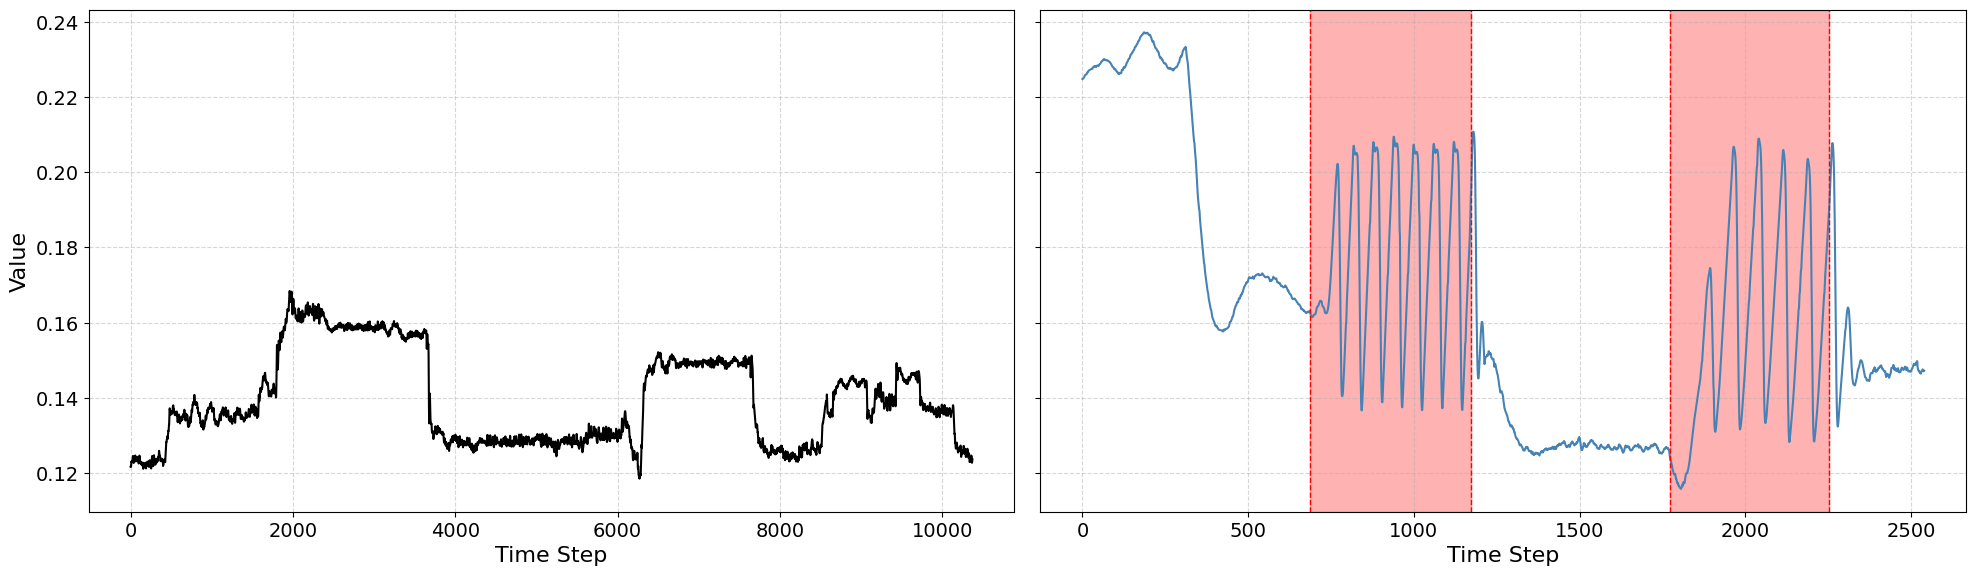
\includegraphics[width=\linewidth]{figures/comparison_F1_T1_vs_FaultyCase5_Set5_1.png}
        \caption{Normal (T1, Feature 1) vs. Slugging (\texttt{FaultyCase5\_Set5\_1}, Feature 1)}\label{fig:comp_5_5_1}
    \end{subfigure}
    \vspace{1em}
    \begin{subfigure}[b]{0.95\linewidth}
        \centering
        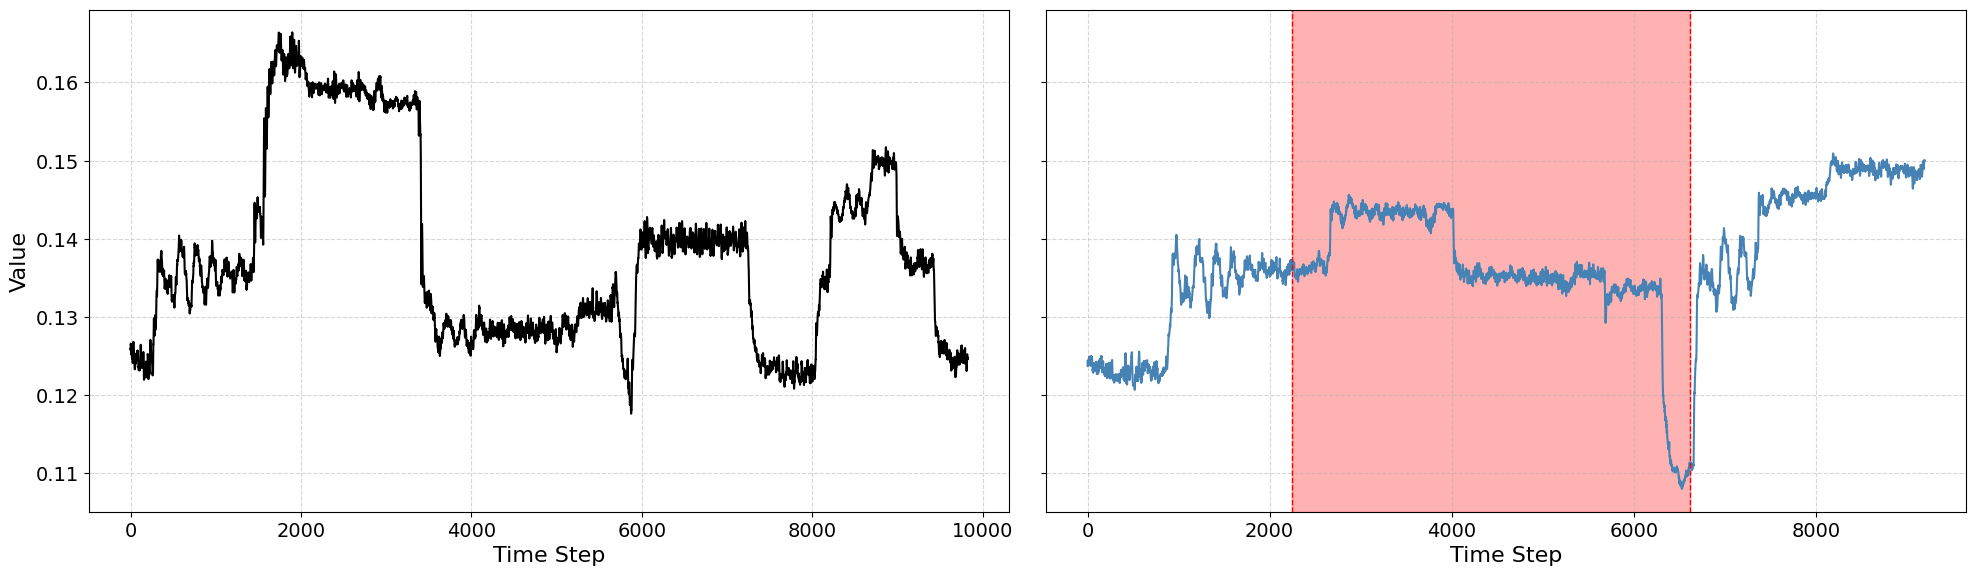
\includegraphics[width=\linewidth]{figures/comparison_F1_T2_vs_FaultyCase2_Set2_1.png}
        \caption{Normal (T2, Feature 1) vs. Water Line Blockage (\texttt{FaultyCase2\_Set2\_1}, Feature 1)}\label{fig:comp_2_2_1}
    \end{subfigure}
    \caption{Representative examples of sensor signals for Feature 1 (pressure), selected to illustrate the model's differential performance. Each subplot compares a normal operation signal (left) with a faulty one (right). Red-shaded regions indicate the ground-truth fault interval. (a) Compares normal operation (T1) with chaotic signature of slugging (\texttt{FaultyCase5\_Set5\_1}), a fault type the model detects effectively. (b) Compares normal operation (T2) with gradual drift characteristic of a water line blockage (\texttt{FaultyCase2\_Set2\_1}), which poses a greater detection challenge.}\label{fig:comparison_signals}
\end{figure}

\paragraph{Analysis of High-Frequency Anomaly Detection (Slugging).}
Figure~\ref{fig:case_5_5_1} exemplifies the model's strength in detecting the slugging conditions in \texttt{FaultyCase5\_Set5\_1}. The energy distribution (Figure~\ref{fig:dist_5_5_1}) shows a clear and wide separation between the low-energy manifold of normal data and the high-energy region of anomalous data. This clean separation corresponds to the high ROC-AUC score (0.94) reported in Table~\ref{tab:model_comparison_f1_auc}, indicating the model has learned a highly discriminative energy function. Consequently, the energy score over time (Figure~\ref{fig:time_5_5_1}) is precise and decisive; it rises at the fault's onset and returns to the normal baseline immediately upon resolution, confirming the model's effectiveness in localizing transient, non-stationary anomalies.

\begin{figure}[h!]
    \centering
    \begin{subfigure}[b]{0.49\linewidth}
        \centering
        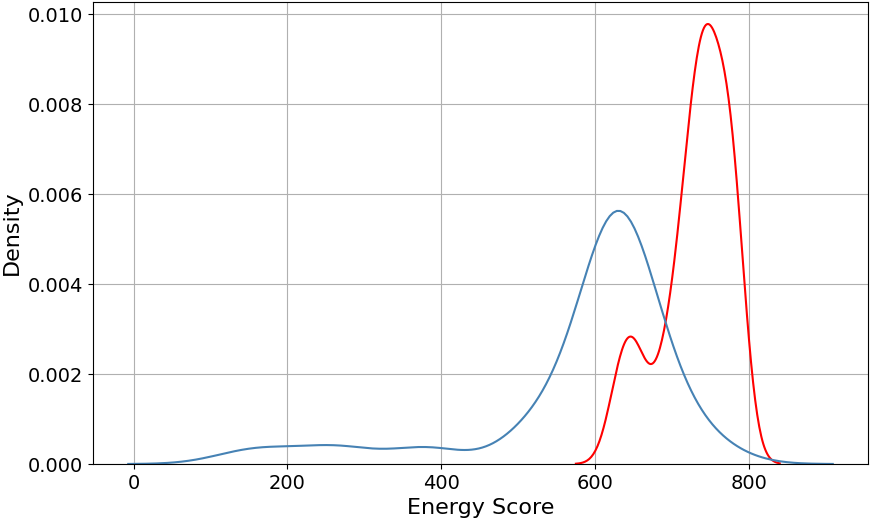
\includegraphics[width=\linewidth]{figures/scores_threshold_energy_distribution_5_5_1.png}
        \caption{Energy distribution (\texttt{FaultyCase5\_Set5\_1})}\label{fig:dist_5_5_1}
    \end{subfigure}
    \hfill
    \begin{subfigure}[b]{0.49\linewidth}
        \centering
        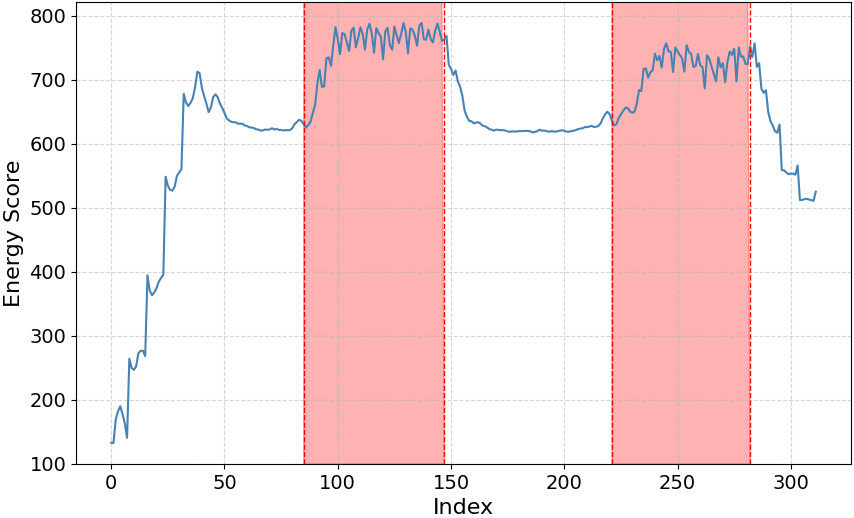
\includegraphics[width=\linewidth]{figures/scores_threshold_energy_over_time_5_5_1.png}
        \caption{Energy score over time (\texttt{FaultyCase5\_Set5\_1})}\label{fig:time_5_5_1}
    \end{subfigure}
    \caption{Qualitative analysis of a successful detection: \texttt{FaultyCase5\_Set5\_1} (Slugging). (a) The energy distributions for normal (blue) and anomalous (red) data are well-separated, corresponding to a high ROC-AUC. (b) The energy score timeline, derived from all input features, shows a sharp, precise response. The red-shaded region indicates the ground-truth fault interval.}\label{fig:case_5_5_1}
\end{figure}

\paragraph{Analysis of Slow-Drift Anomaly Detection (Blockage).} \label{sec:slow_drift_analysis}
In contrast, Figure~\ref{fig:case_2_2_1} depicts the model's struggles with the gradual water line blockage in \texttt{FaultyCase2\_Set2\_1}. The energy distribution (Figure~\ref{fig:dist_2_2_1}) reveals limited separability for this fault type. Instead of assigning consistently higher energy to the anomaly, the model produces heavily overlapping distributions where the anomalous scores (red) are not clearly separated to the right of the normal scores (blue). This indicates that the learned energy function is not discriminative for this type of deviation, which directly explains the near-random ROC-AUC score (0.37) for this case (Table~\ref{tab:model_comparison_f1_auc}). The energy timeline (Figure~\ref{fig:time_2_2_1}) further exposes this limitation; instead of a prompt response, the model's energy score remains low during the initial fault phase and rises only gradually. This delayed and weaker response degrades detection performance and highlights the model's difficulty with slowly evolving deviations.

\begin{figure}[h!]
    \centering
    \begin{subfigure}[b]{0.49\linewidth}
        \centering
        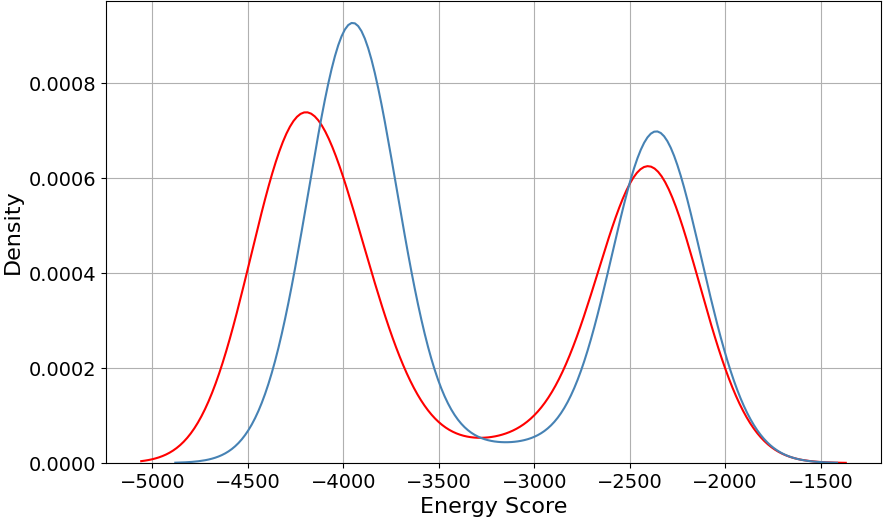
\includegraphics[width=\linewidth]{figures/scores_threshold_energy_distribution_2_2_1.png}
        \caption{Energy distribution (\texttt{FaultyCase2\_Set2\_1})}\label{fig:dist_2_2_1}
    \end{subfigure}
    \hfill
    \begin{subfigure}[b]{0.49\linewidth}
        \centering
        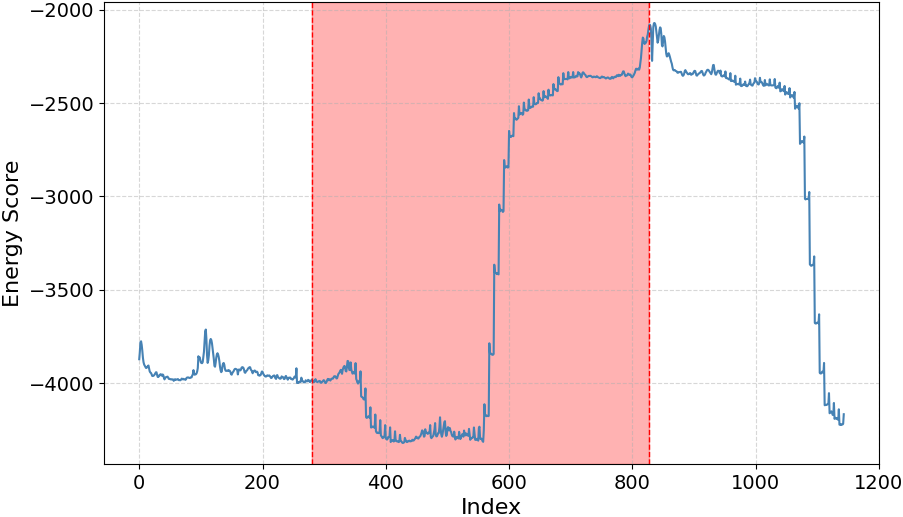
\includegraphics[width=\linewidth]{figures/scores_threshold_energy_over_time_2_2_1.png}
        \caption{Energy score over time (\texttt{FaultyCase2\_Set2\_1})}\label{fig:time_2_2_1}
    \end{subfigure}
    \caption{Qualitative analysis of a challenging detection: \texttt{FaultyCase2\_Set2\_1} (Blockage). (a) The energy distributions are heavily overlapped, leading to a low ROC-AUC. (b) The energy score timeline, derived from all input features, shows a delayed and weak response. The red-shaded region indicates the ground-truth fault interval.}\label{fig:case_2_2_1}
\end{figure}


\section{Discussion}\label{sec:discussion}

\subsection{Implications and Insights}

Our results highlight several design principles for anomaly detection in complex industrial processes.

\paragraph{Representation matters as much as architecture.}
Performance on chaotic, high-frequency faults (e.g., FaultyCase 5) shows that transforming 1D signals into 2D time–frequency images via the CWT can convert a hard temporal problem into a textural pattern-recognition task, where Vision Transformers excel. Rather than replacing feature engineering, modern architectures benefit from representational choices that align with their inductive biases.

\paragraph{Architectural specialization is beneficial.}
Comparisons with the LSTM baseline suggest complementary strengths: recurrent models favor long-range, quasi-periodic patterns (FaultyCase 3), while our patch-based approach is strong for localized, non-stationary events (FaultyCase 5). This pattern argues for ensembles or hybrids that combine recurrent and attention-based components, rather than seeking a single model that dominates across all anomaly types.

\paragraph{EBMs separate anomaly scoring from decision-making.}
Cases with high ROC-AUC but lower F1 indicate that the energy function can be discriminative while a static decision threshold underperforms. This separation is useful: the EBM provides a principled anomaly score, and thresholding can be improved independently (e.g., via adaptive or sequential methods).

\subsection{Limitations}

\paragraph{Sensitivity to slow-drift anomalies.}
The most salient weakness is reduced sensitivity to slowly evolving faults (e.g., \texttt{FaultyCase2\_Set2\_1}, Section~\ref{sec:slow_drift_analysis}). Two factors contribute: (i) when detrending is applied, it can attenuate gradual deviations by design; and (ii) the ViT processes fixed-size chunks without recurrent memory, making subtle, long-horizon changes harder to detect. This manifests as delayed energy increases and overlapping score distributions (Figure~\ref{fig:case_2_2_1}).

\paragraph{Compute and hyperparameter sensitivity.}
CWT preprocessing and Energy Matching with a ViT are more resource-intensive than operating on raw signals, and performance depends on context length. As shown in our chunk-width analysis (Section~\ref{sec:chunk_size_analysis}), the optimal window balances modeling longer normal dynamics against sensitivity to short-lived faults, implying nontrivial tuning for new deployments.

\paragraph{Diagnostic interpretability.}
Energy maps localize anomalies in time–frequency space but do not attribute root-cause sensors directly. Because channels are concatenated and scored jointly, attributing a high-energy patch to specific inputs requires post-hoc analysis. Resolution is also bounded by the patch size, limiting sub-patch localization needed for fine-grained diagnosis.

\subsection{Future Work}

\paragraph{Hybrid models for multi-scale dynamics.}
Augment ScaloVit-EBM with a lightweight recurrent branch (e.g., LSTM/GRU) over raw or downsampled signals and fuse outputs, targeting robustness to both slow drifts and high-frequency events.

\paragraph{Attribution and hierarchical localization.}
Develop gradient-based or attention-driven attributions to relate high-energy regions to input channels, and trigger secondary, finer-grained analysis on high-energy patches to achieve sub-patch localization.

\paragraph{Adaptive and online deployment.}
Enable streaming operation with efficient, stateful CWT and adopt adaptive decision rules (e.g., change-point detection, Bayesian or percentile policies with drift correction) to maintain performance under nonstationarity.

\section{Conclusion}

This work presented ScaloVit-EBM, a localized energy-based model for unsupervised anomaly detection in multivariate industrial time series. By converting sensor streams into multichannel CWT scalograms and learning per-patch energies with a U-Net plus Vision Transformer backbone trained via Energy Matching on normal-only data, the method produces interpretable time–frequency energy maps and a principled anomaly score. A deployment-minded inference protocol—overlapping chunking with max aggregation and a percentile threshold calibrated on normal validation—keeps scoring and decision-making decoupled and simple to operate.

On a realistic three-phase flow benchmark, ScaloVit-EBM is competitive with or superior to strong reconstruction- and Transformer-based baselines, and excels on high-frequency slugging where localized time–frequency structure is critical. Ablations substantiate three practical design choices: detrending improves class separability; max aggregation avoids diluting localized deviations across overlaps; and chunk width trades off long-range context against sensitivity to short-lived events. Additional analyses show that localized, per-patch scoring is important for spatially complex faults, while augmenting the objective with Contrastive Divergence can improve F1 at the expense of ROC-AUC and training cost.

Limitations include reduced sensitivity to gradually evolving faults, dependence on chunk length and preprocessing, and limited channel-level attribution. These motivate extensions toward hybrid recurrent–attention architectures for multi-scale dynamics, hierarchical and channel-aware attribution mechanisms, and adaptive, streaming deployment to handle nonstationarity.

\section*{Acknowledgments}
We would like to express our sincere gratitude to our main supervisor, Dr. Loo Junn Yong, and co-supervisor, Dr. Ting Chee Ming, for their invaluable guidance and support throughout this research. We also extend our thanks to Tew Hwa Hui for the fruitful discussions and cooperation.
This work made use of the Three-Phase Flow Facility dataset, generously provided by Cranfield University \citep{cao_mba_lao_samuel_2015}. The implementation of our energy-based model is adapted from the official Energy Matching codebase provided by Balcerak et al. in their public repository \citep{balcerak2025energymatchingunifyingflow}. Furthermore, our signal preprocessing methodology was informed by the techniques presented in the ImagenTime project by \cite{naiman_berman_pemper_arbiv_fadlon_azencot_2024}. 

\bibliographystyle{plainnat}
\bibliography{references}

\section*{Appendix}
\input{appendices/appendix.tex}

\end{document}